% TeX encoding = utf8
% TeX spellcheck = pl_PL 
\documentclass[a4paper, 11pt]{article}
\usepackage[utf8]{inputenc}
\usepackage[polish]{babel}
\usepackage{polski}
\usepackage{float}
\usepackage{graphicx}
\usepackage{listings}
\usepackage{amsfonts}
\usepackage{geometry}
\usepackage{multicol}
\usepackage{latexsym}
\usepackage{enumerate}
\usepackage{hyperref}
\usepackage{wrapfig}
\usepackage{color} %red, green, blue, yellow, cyan, magenta, black, white
\definecolor{mygreen}{RGB}{28,172,0} % color values Red, Green, Blue
\definecolor{mylilas}{RGB}{170,55,241}

\author{Kamil Foryszewski}
\title{Modelowanie i identyfkacja - projekt II, zadanie 9}
\frenchspacing

\newgeometry{tmargin=2cm, bmargin=2cm, lmargin=2cm, rmargin=2cm}
\pagestyle{empty}


\begin{document}

\lstset{language=Matlab,%
    basicstyle=\color{red},
    breaklines=true,%
    morekeywords={matlab2tikz},
    keywordstyle=\color{blue},%
    morekeywords=[2]{1}, keywordstyle=[2]{\color{black}},
    identifierstyle=\color{black},%
    stringstyle=\color{mylilas},%
    commentstyle=\color{mygreen},%
    showstringspaces=false,
    numbers=right,%
    numberstyle={ \color{black}},% size of the numbers
    numbersep=5pt, % this defines how far the numbers are from the text
    emph=[1]{for,endfor,endwhile,endfunction,endif,break},emphstyle=[1]\color{blue}, %some words to emphasise
    emph=[2]{,.}, emphstyle=[2]\color{yellow},%
}

\maketitle
\tableofcontents

\section{Identyfikacja modelu statycznego}
Skrypt p=w środowisku Matlab wykonujący operacje na dancyh znajduje się w pliku statyczne.m
\subsection{Wykres danych ststycznych}
\begin{figure}[H]
\centering
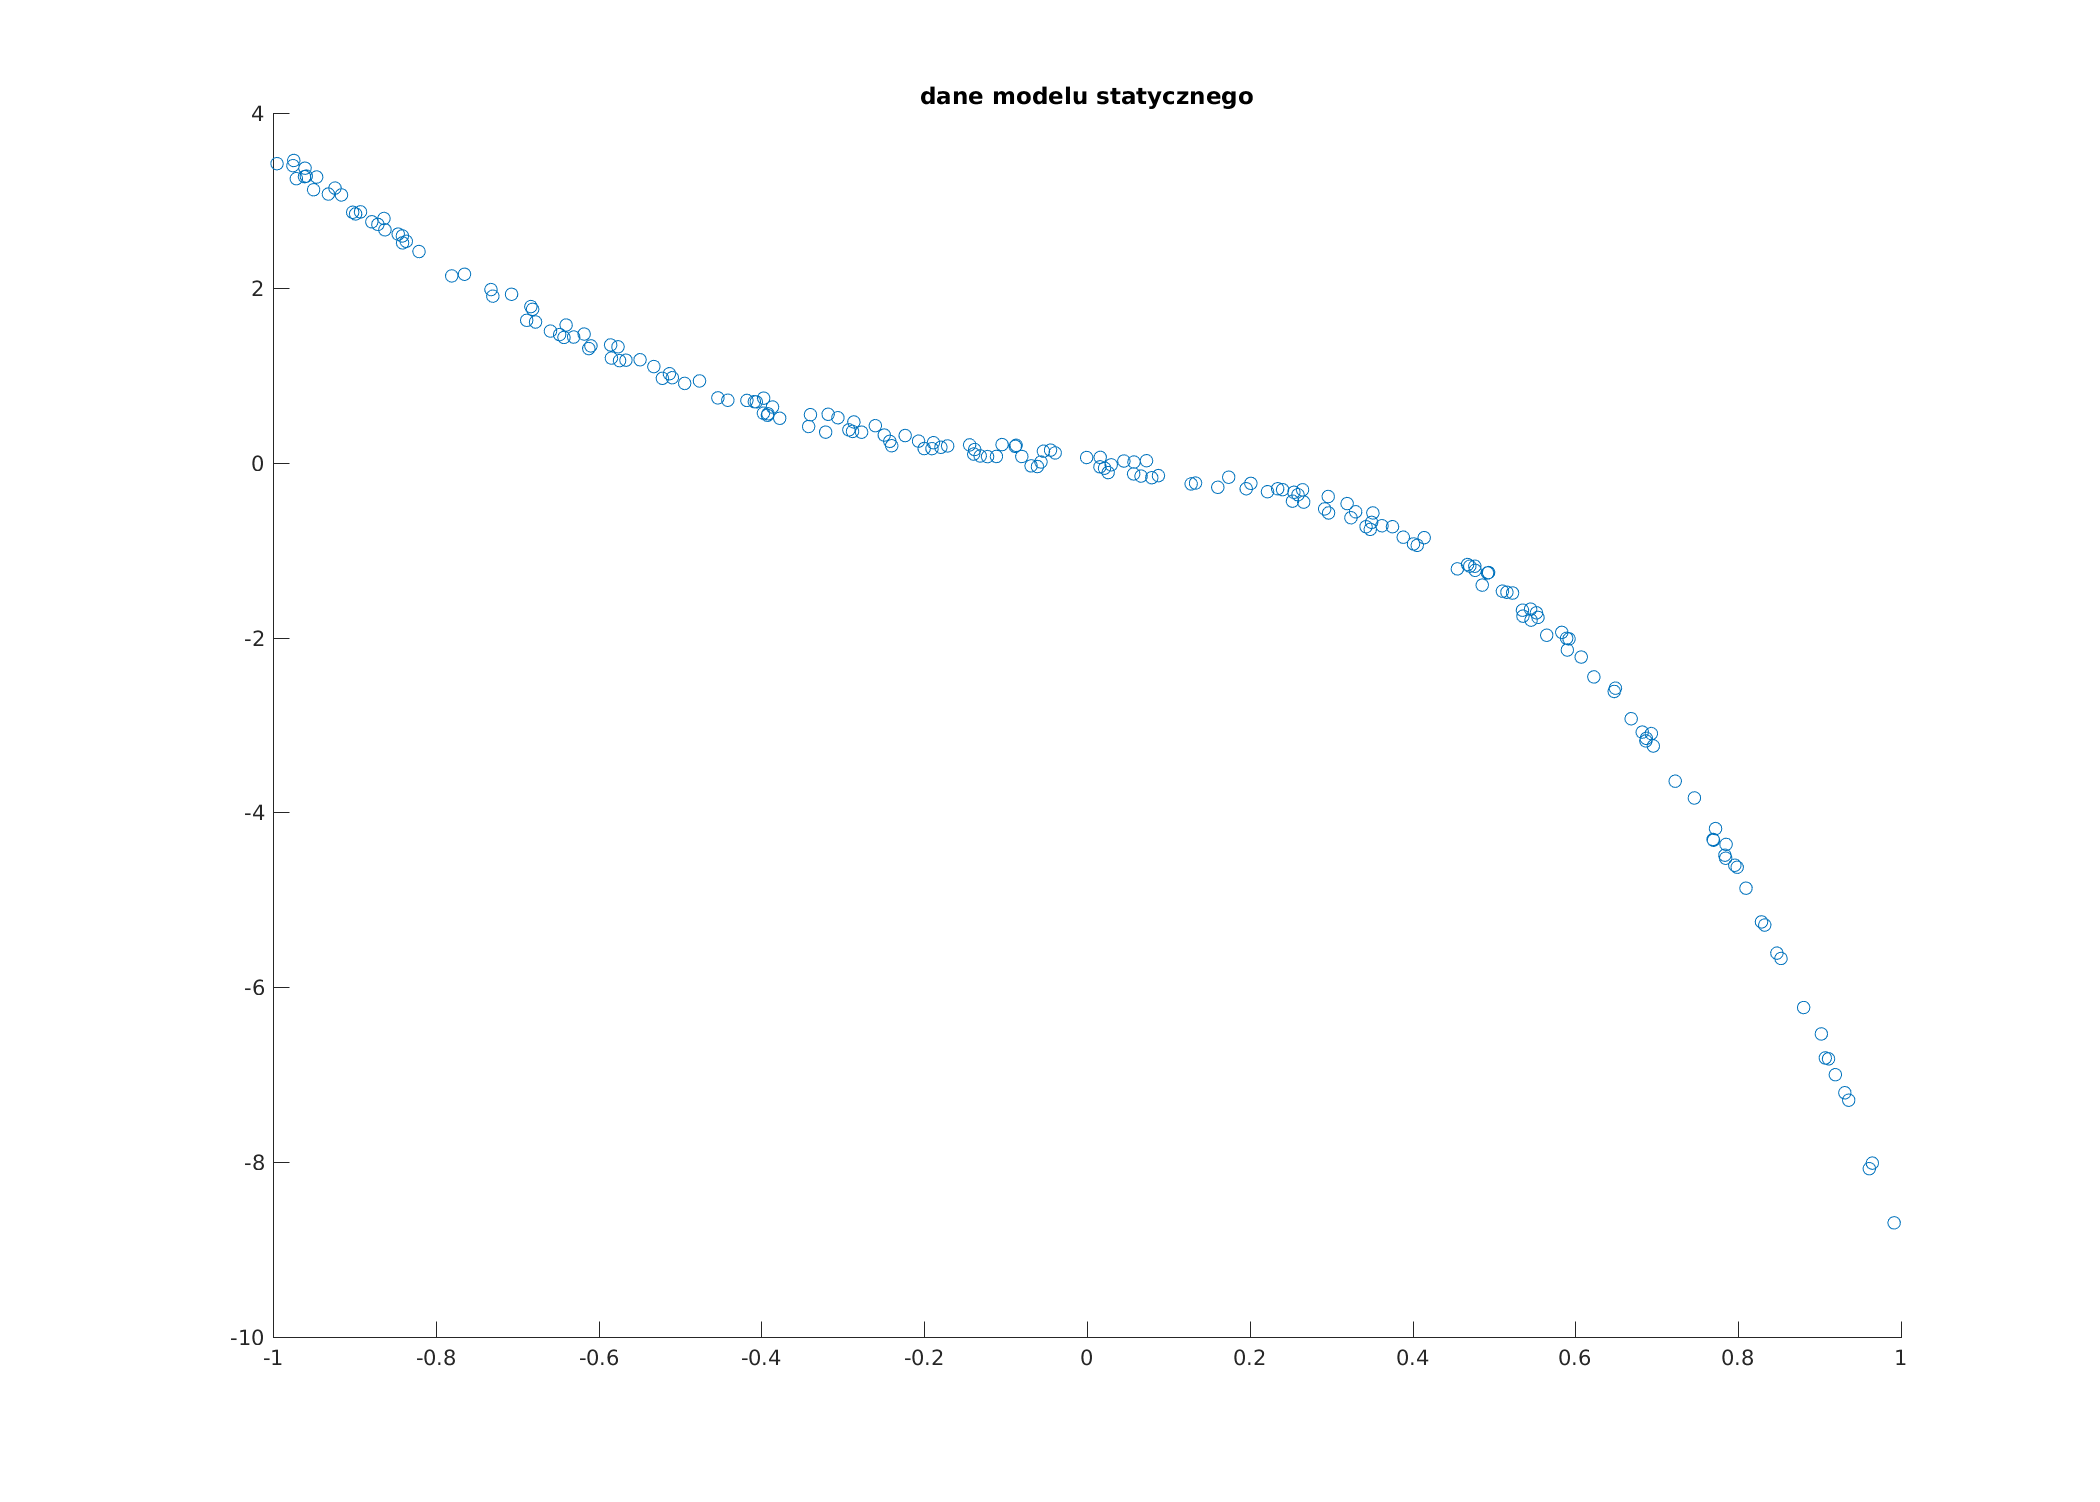
\includegraphics[scale=0.5]{dane_stat.png}
\caption{Zbiór danych statycznych}
\label{}
\end{figure}
\subsection{Podział daych statycznych na zbiory}
Dane statyczne zostały podzielone na zbiory: uczący i weryfikujący poprzez podział na parzyste i nieparzyste próbki. Dane uczące składają się z próbek parzystych, natiomiast weryfikujące z próbek nieparzystych. 
\subsubsection{Reprezentacja graficzna zbioru uczącego}
\begin{figure}[H]
\centering
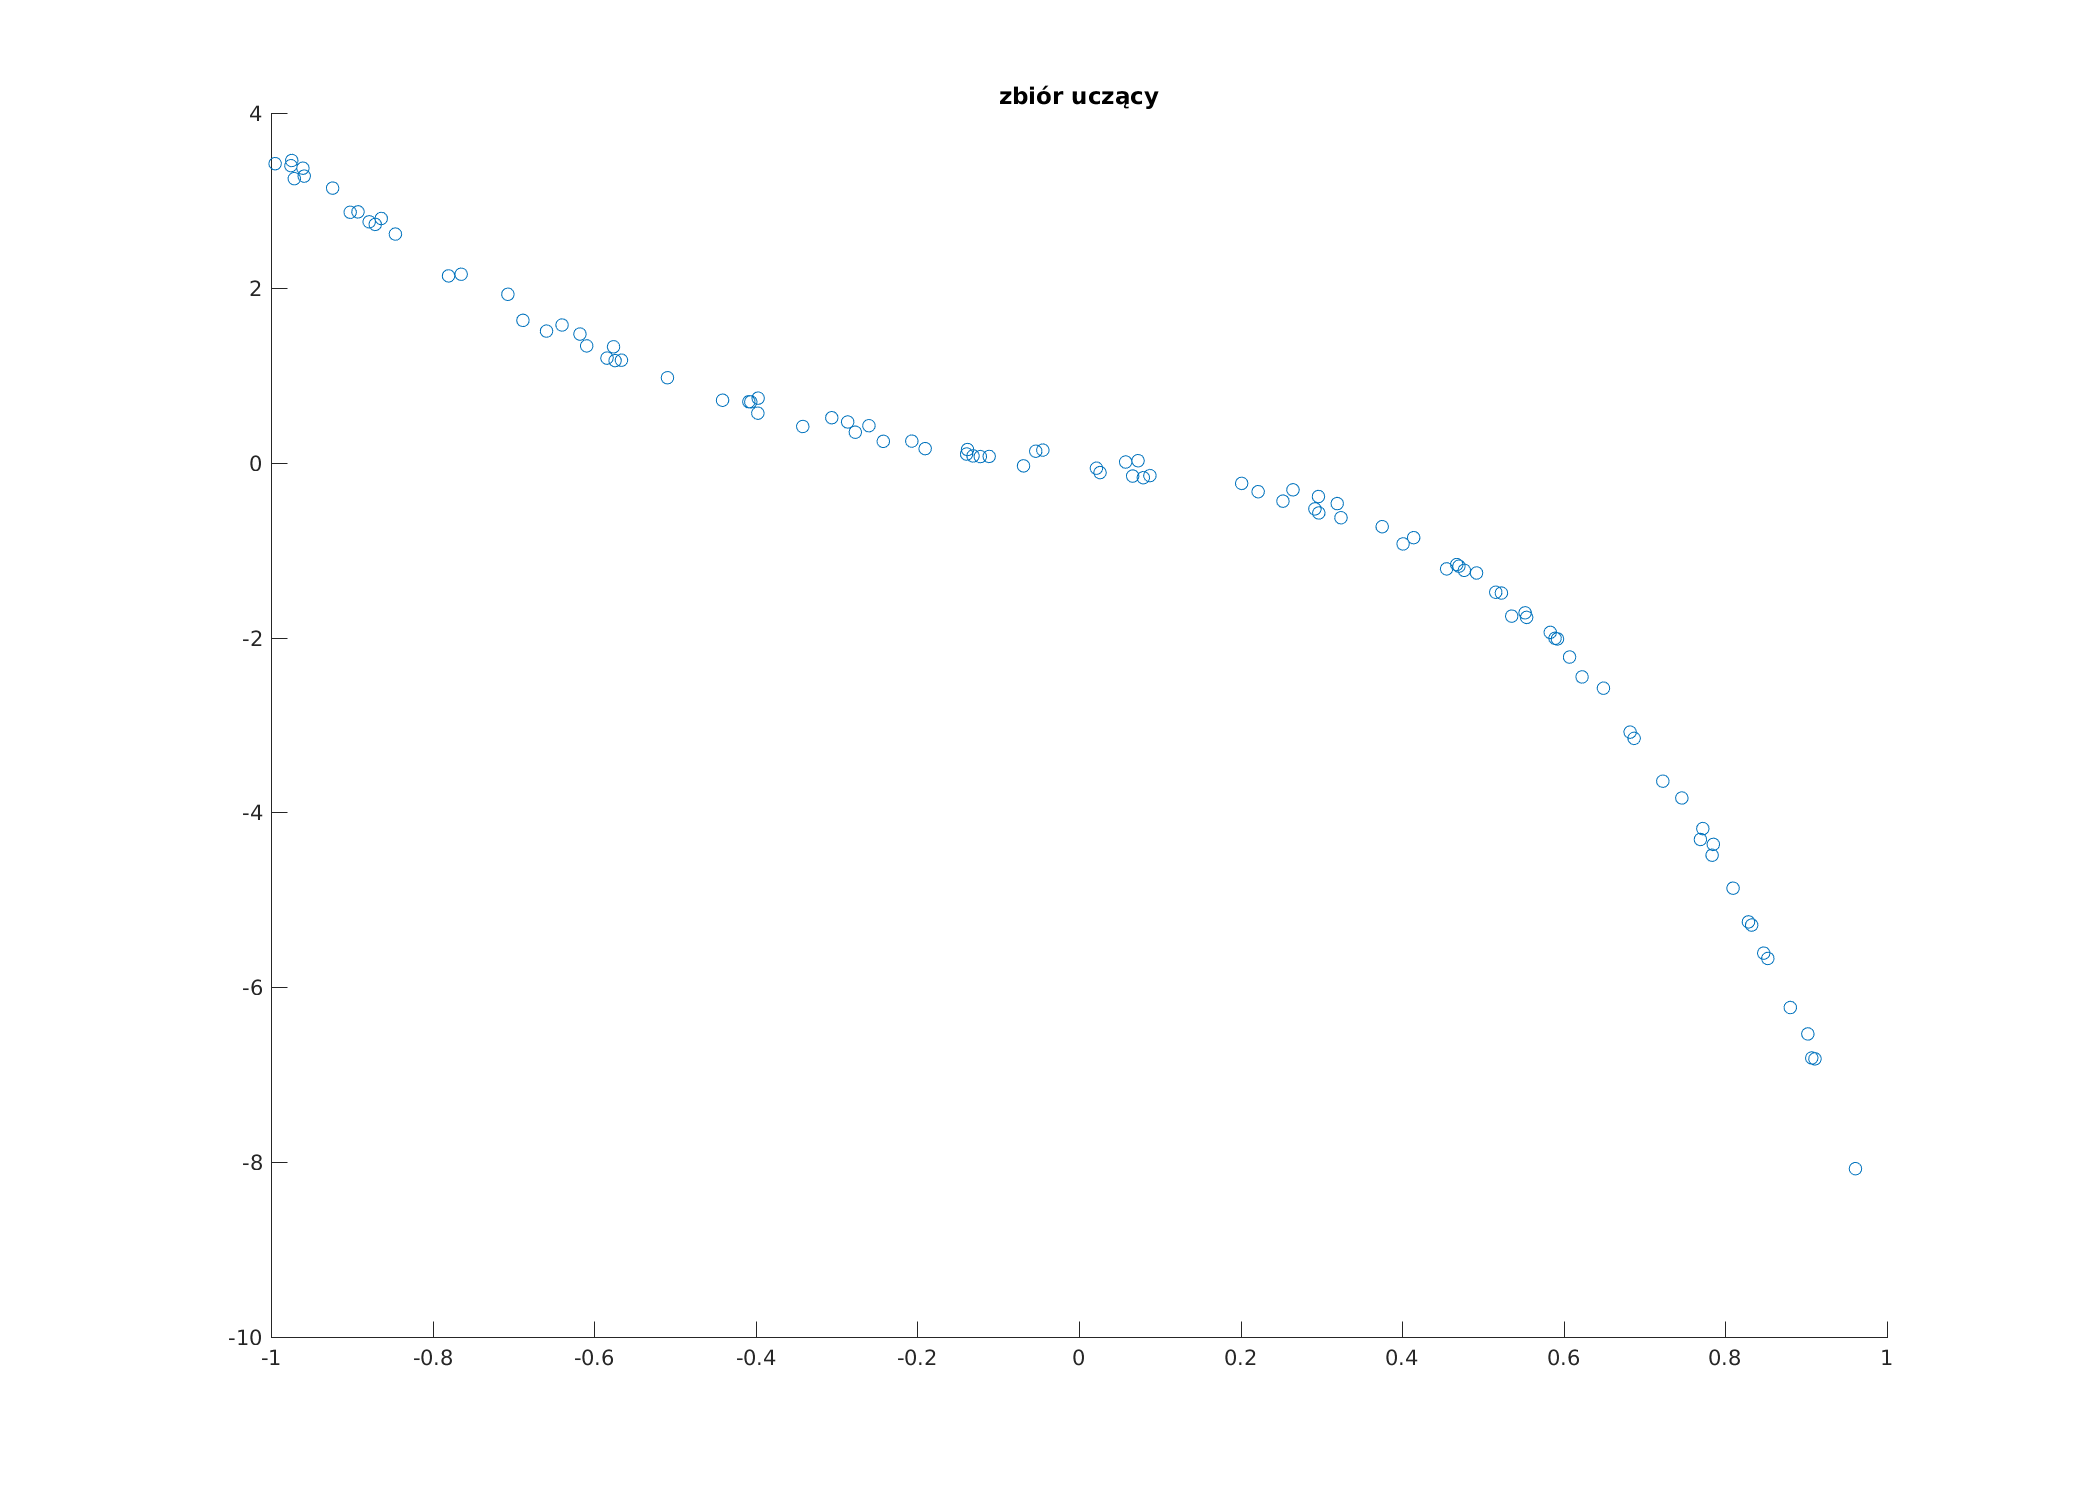
\includegraphics[scale=0.50]{dane_stat_ucz.png}
\caption{Zbiór dancyh uczących }
\label{}
\end{figure}
\subsubsection{reprezentacj graficzna zbioru weryfikującego}
\begin{figure}[H]
\centering
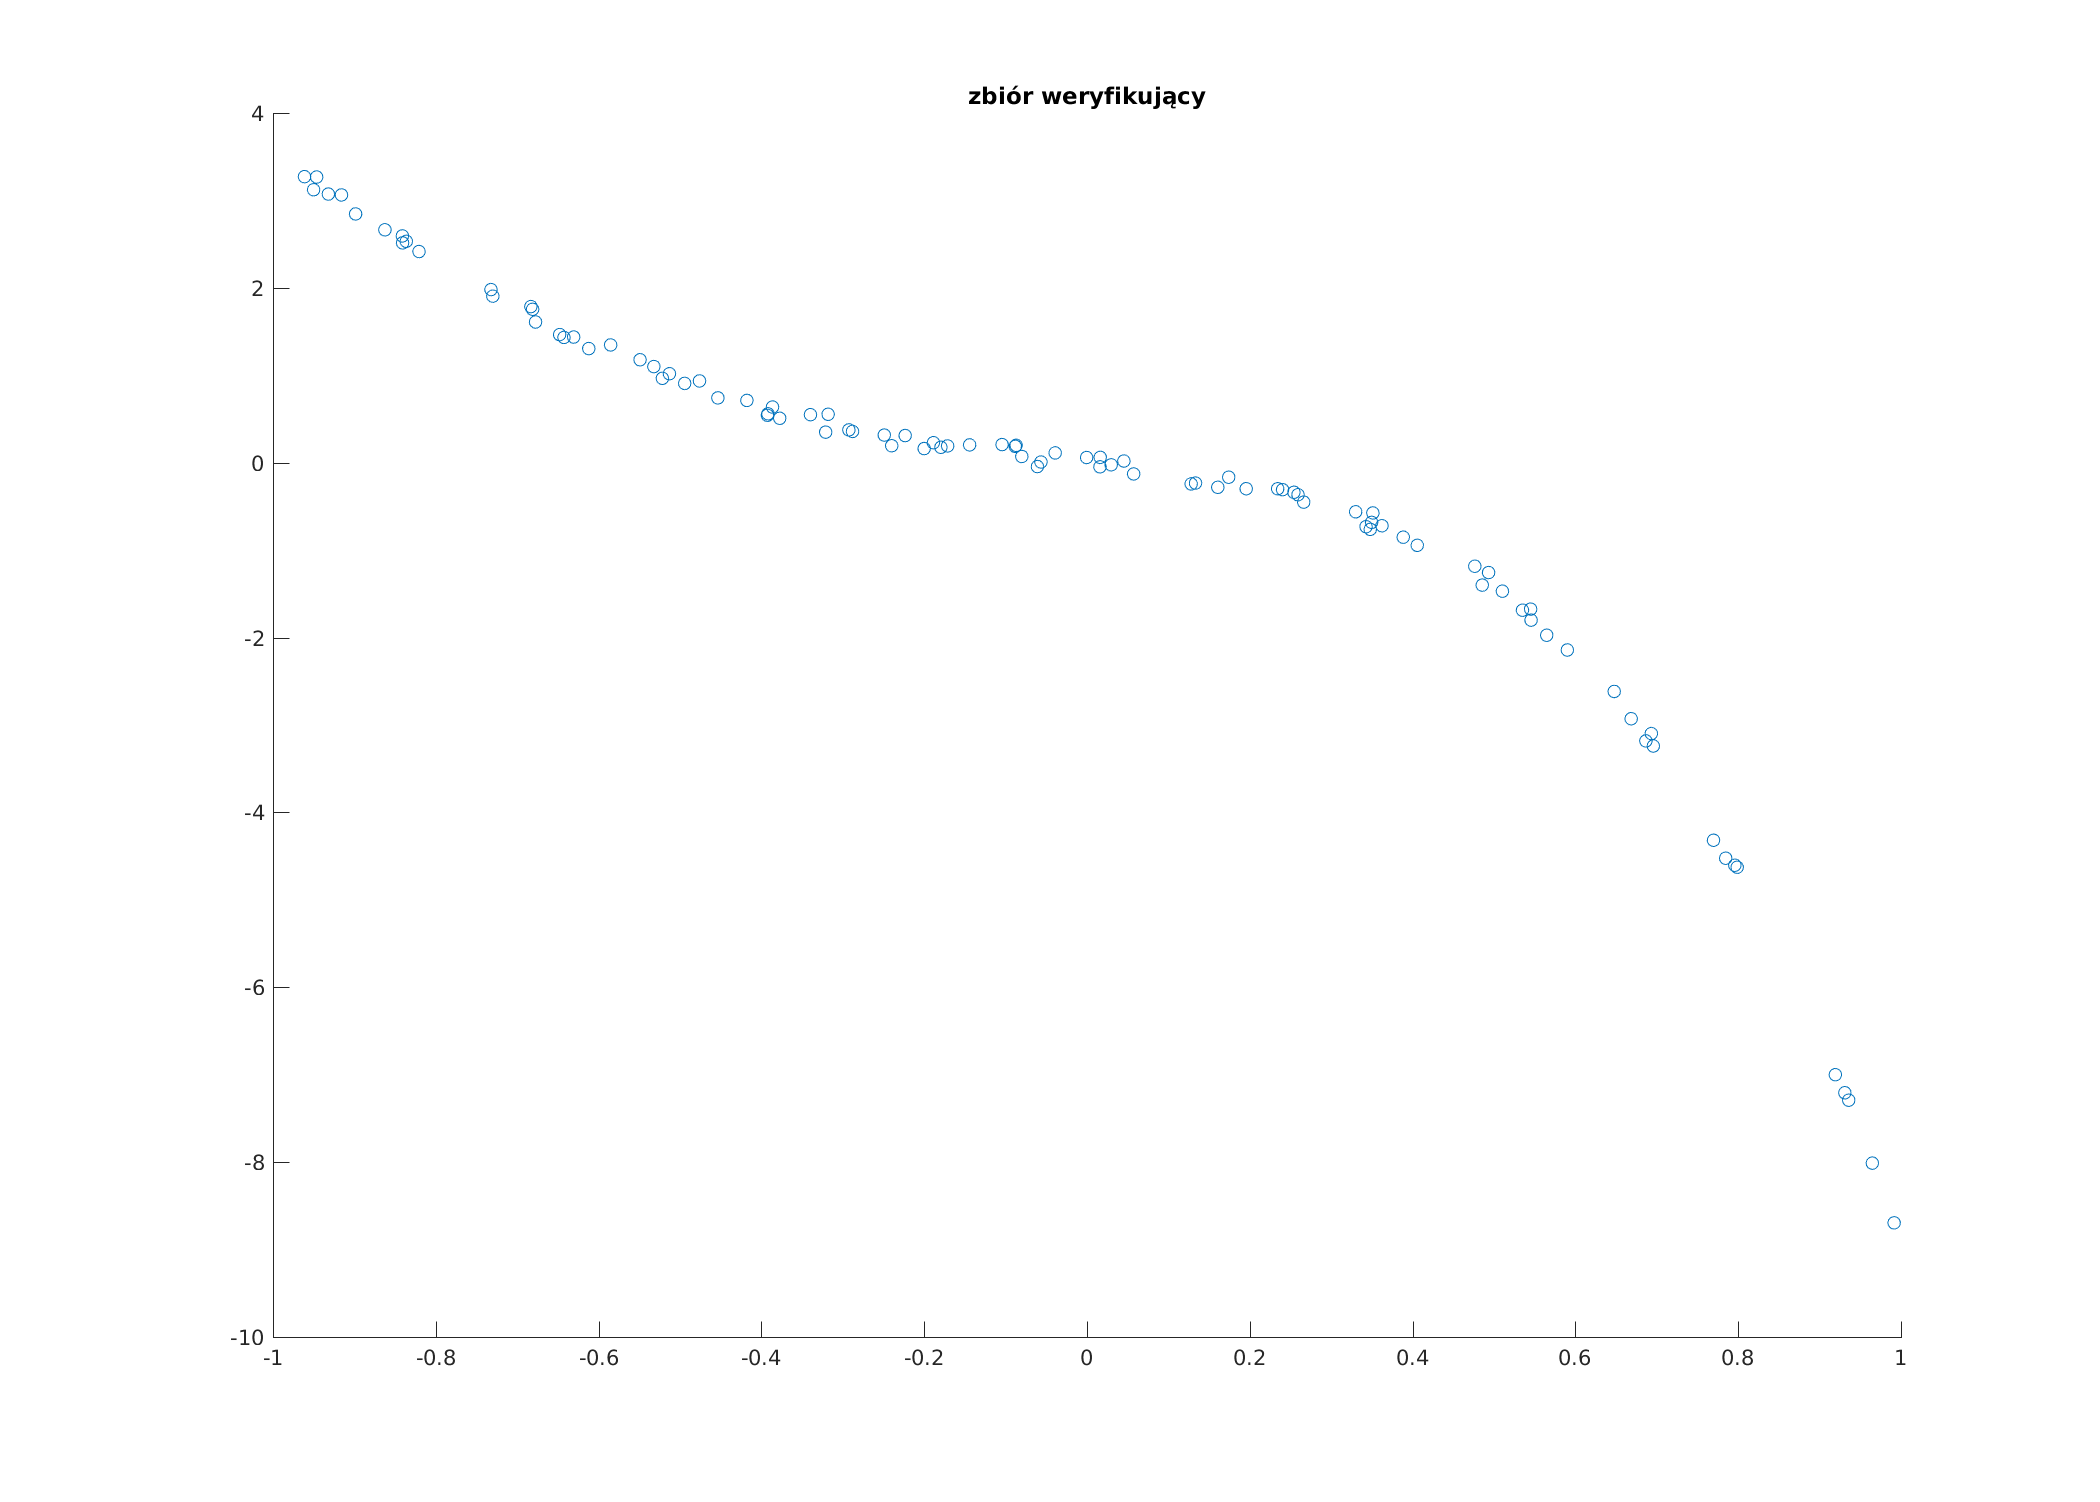
\includegraphics[scale=0.50]{dane_stat_wer.png}
\caption{Zbiór dancyh weryfikujących }
\label{}
\end{figure}
\subsection{Model liniowy}
Ogóna postać modelu lioniowego wygląda następująco: 
$$y(u) = a_1u + a_2$$
Dla danych z zadania została wyznaczona metodą najmniejszych kwadratów i wynosi: 
$$y(u) =-4.039918564118059u -0.514971764481714  $$
\subsubsection{Wykresy charakterystyk modelu liniowego}
Poniżej znajduje się reprezentacja graficzna modelu na tle danych uczących i weryfikujących 
\subsubsection{Wykres charakterystyki na tle zbiorów danych}
\begin{figure}[H]
\centering
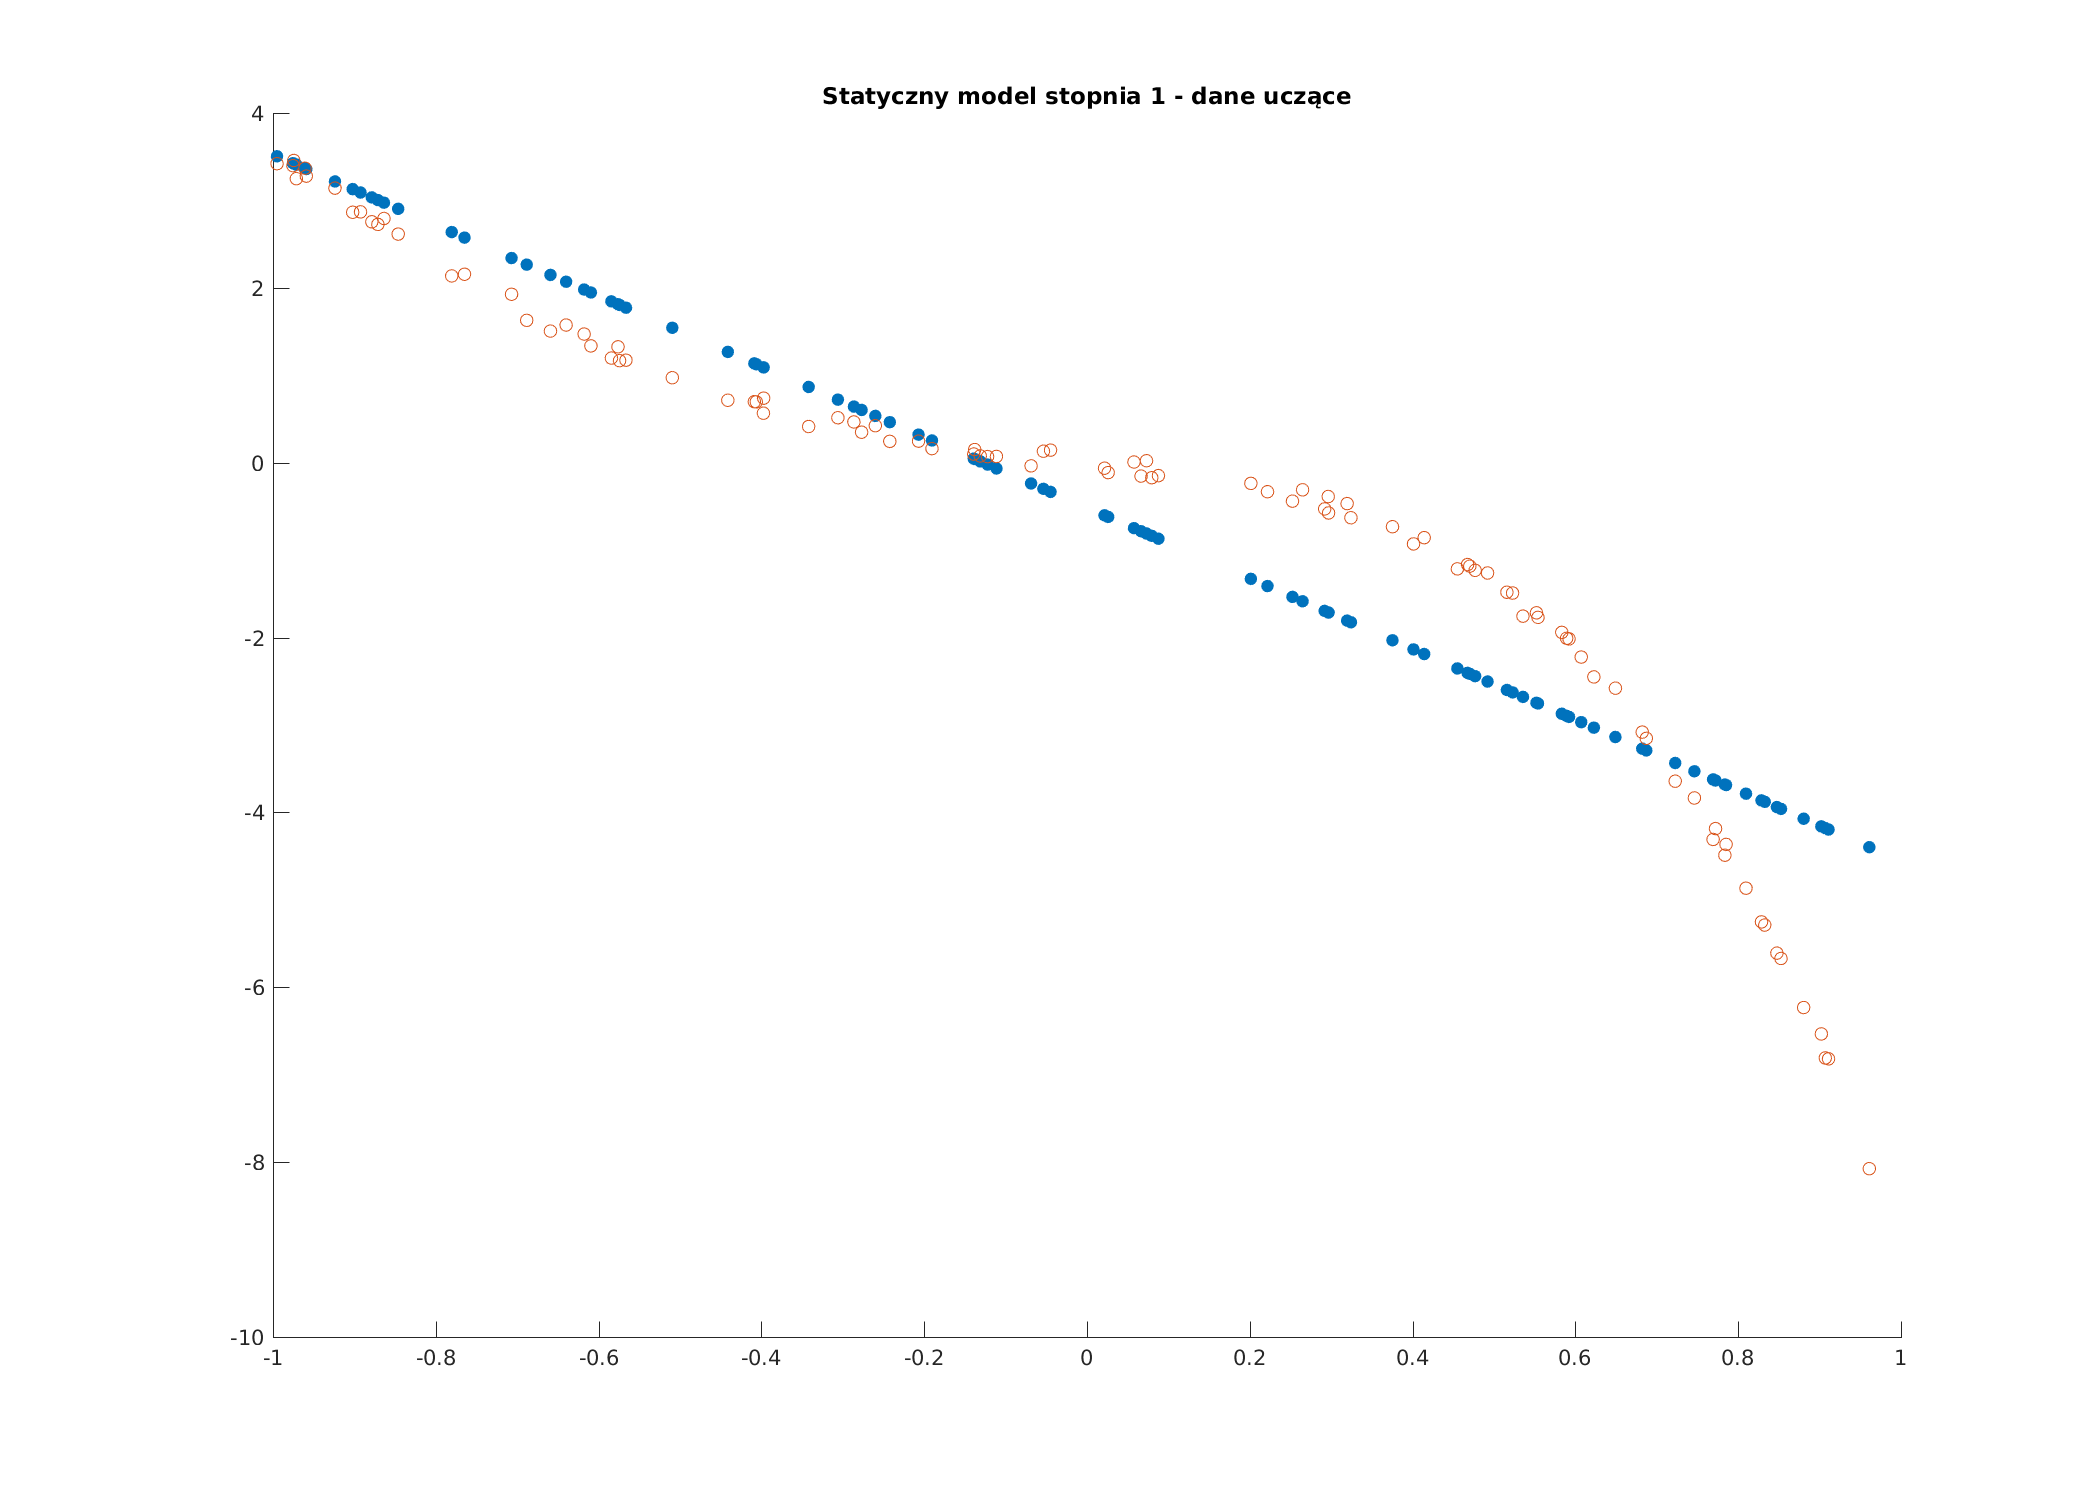
\includegraphics[scale=0.50]{dane_stat_1_ucz.png}
\caption{Charakterystyka modelu na tle zbioru danych uczących}
\label{}
\end{figure}
\begin{figure}[H]
\centering
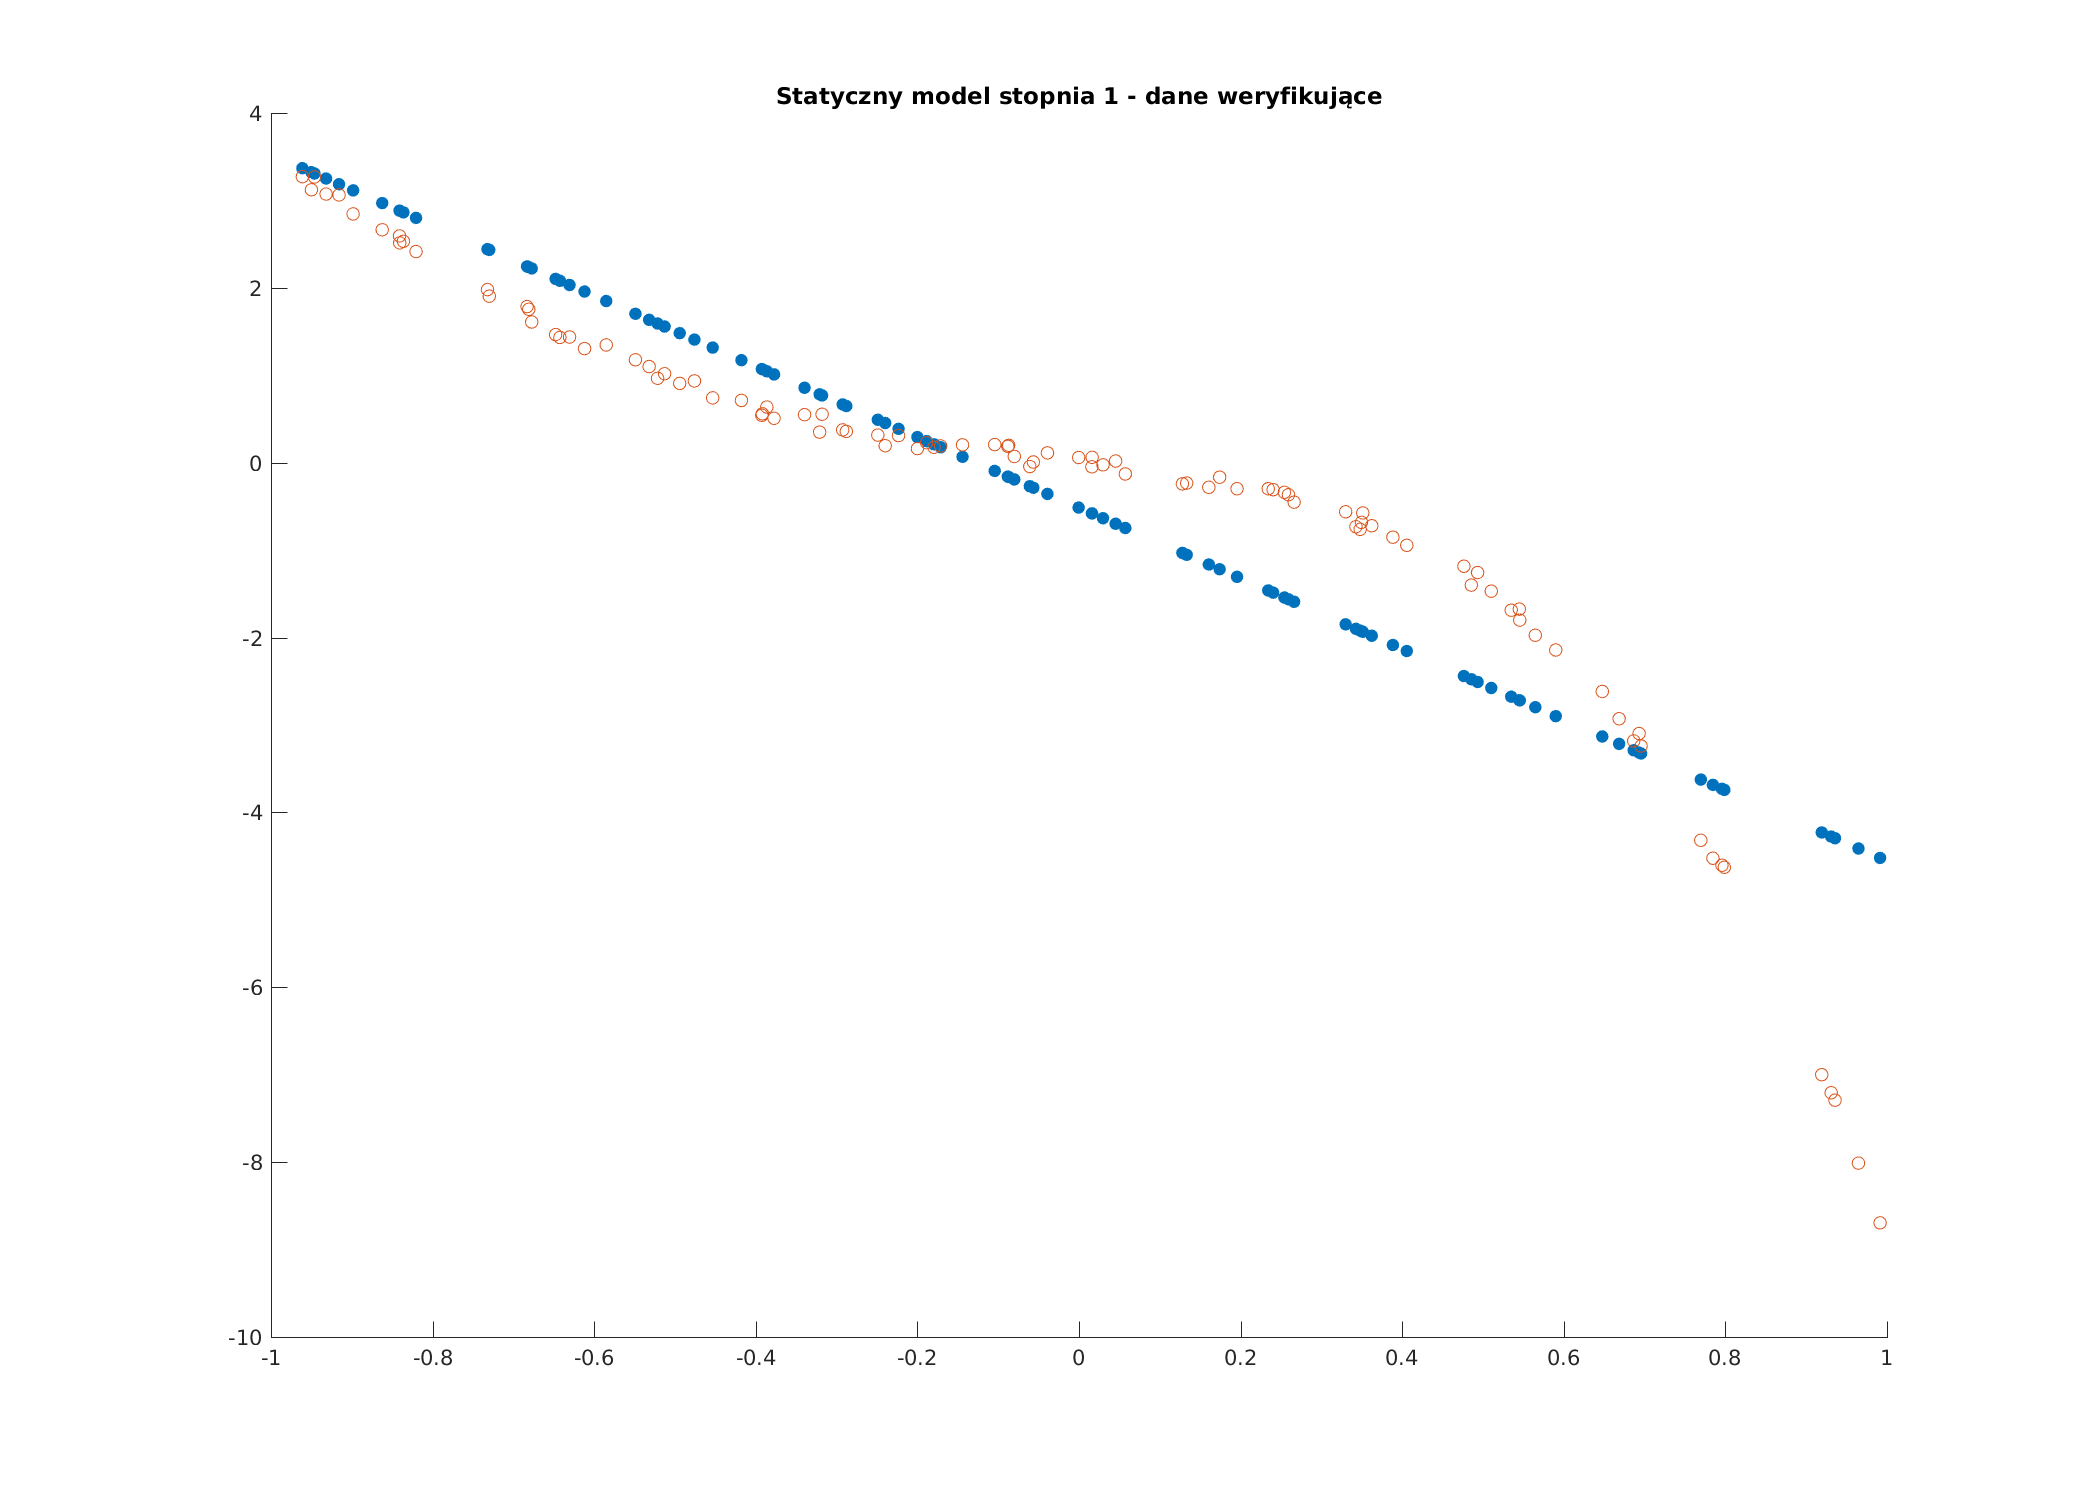
\includegraphics[scale=0.50]{dane_stat_1_wer.png}
\caption{Charakterystyka modelu na tle zbioru danych weryfikujących }
\label{}
\end{figure}
\subsubsection{Błędy zbiorów}

\begin{figure}[H]
\centering
\begin{tabular}{|c|c|c|}
\hline
	N & Błąd dla danych uczących & Bąłd dla danych weryfikujących\\
\hline
	1 & 9.432614 & 1.028\\
\hline
\end{tabular}
\caption{Błędy modelu liniowego}
\end{figure}
\subsection{Statyczne modele nielioniwe}
Dla danych z zadania model niniowy mało dokładnie odwzorowuje poszczególne próbki, dlatego kolejnym krokiem jest zyznaczenie modeli wyższego stopnia. 
\subsubsection{Model stopnia drugiego}
\begin{figure}[H]
\centering
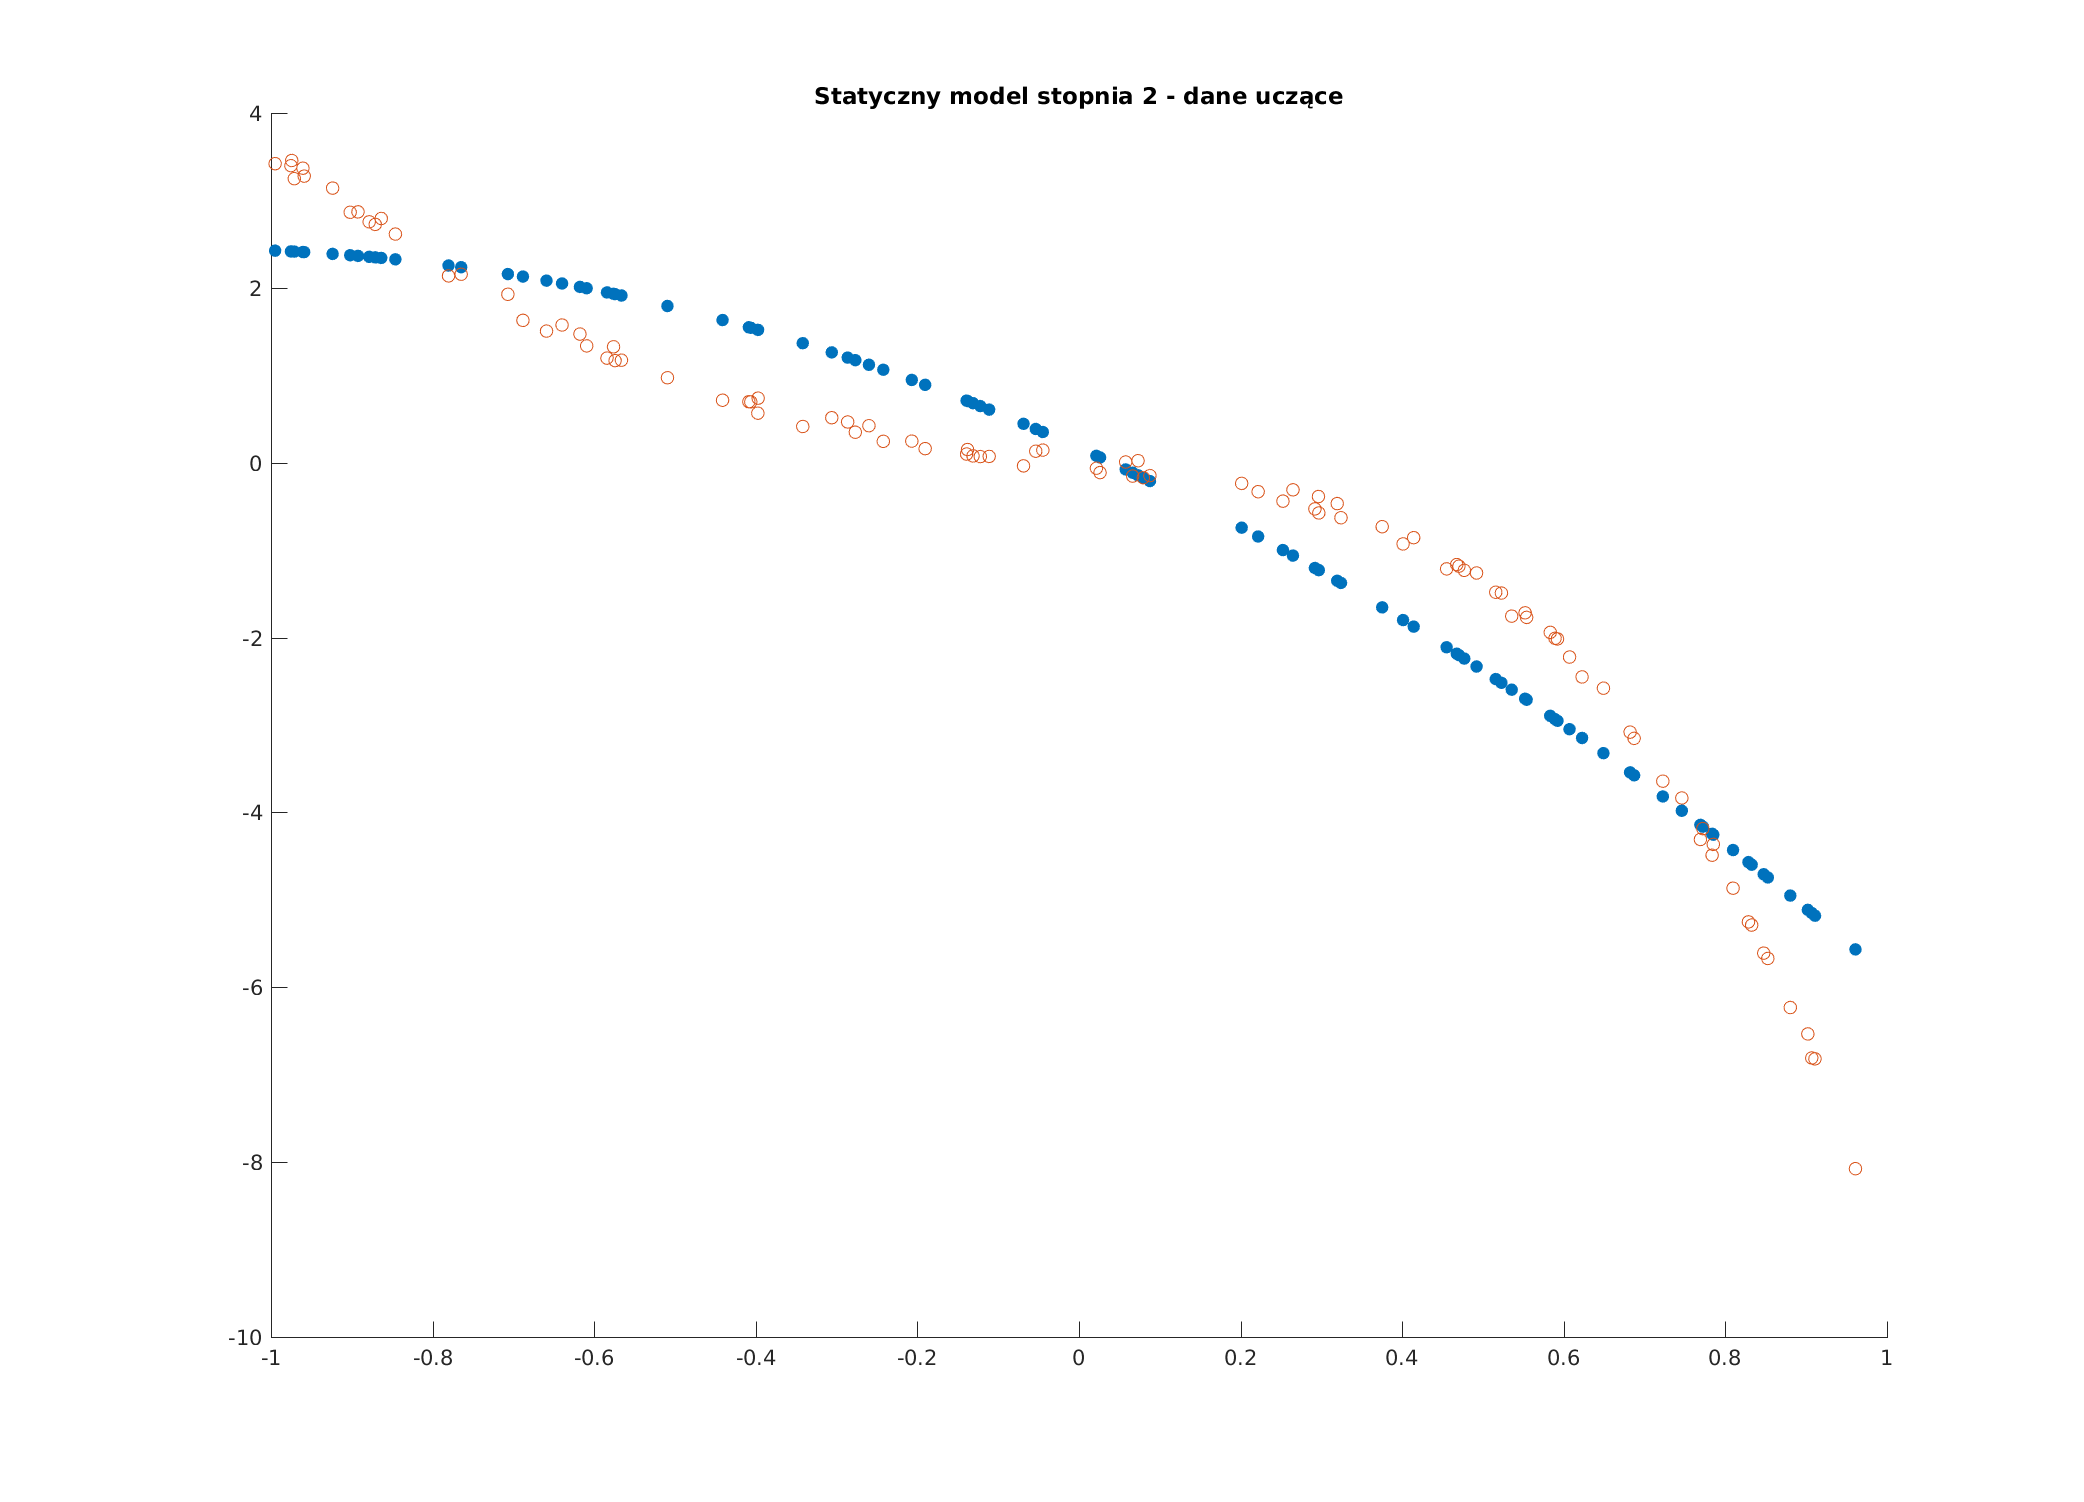
\includegraphics[scale=0.50]{dane_stat_2_ucz.png}
\caption{Model stopnia drugiego dane uczące}
\label{}
\end{figure}
\begin{figure}[H]
\centering
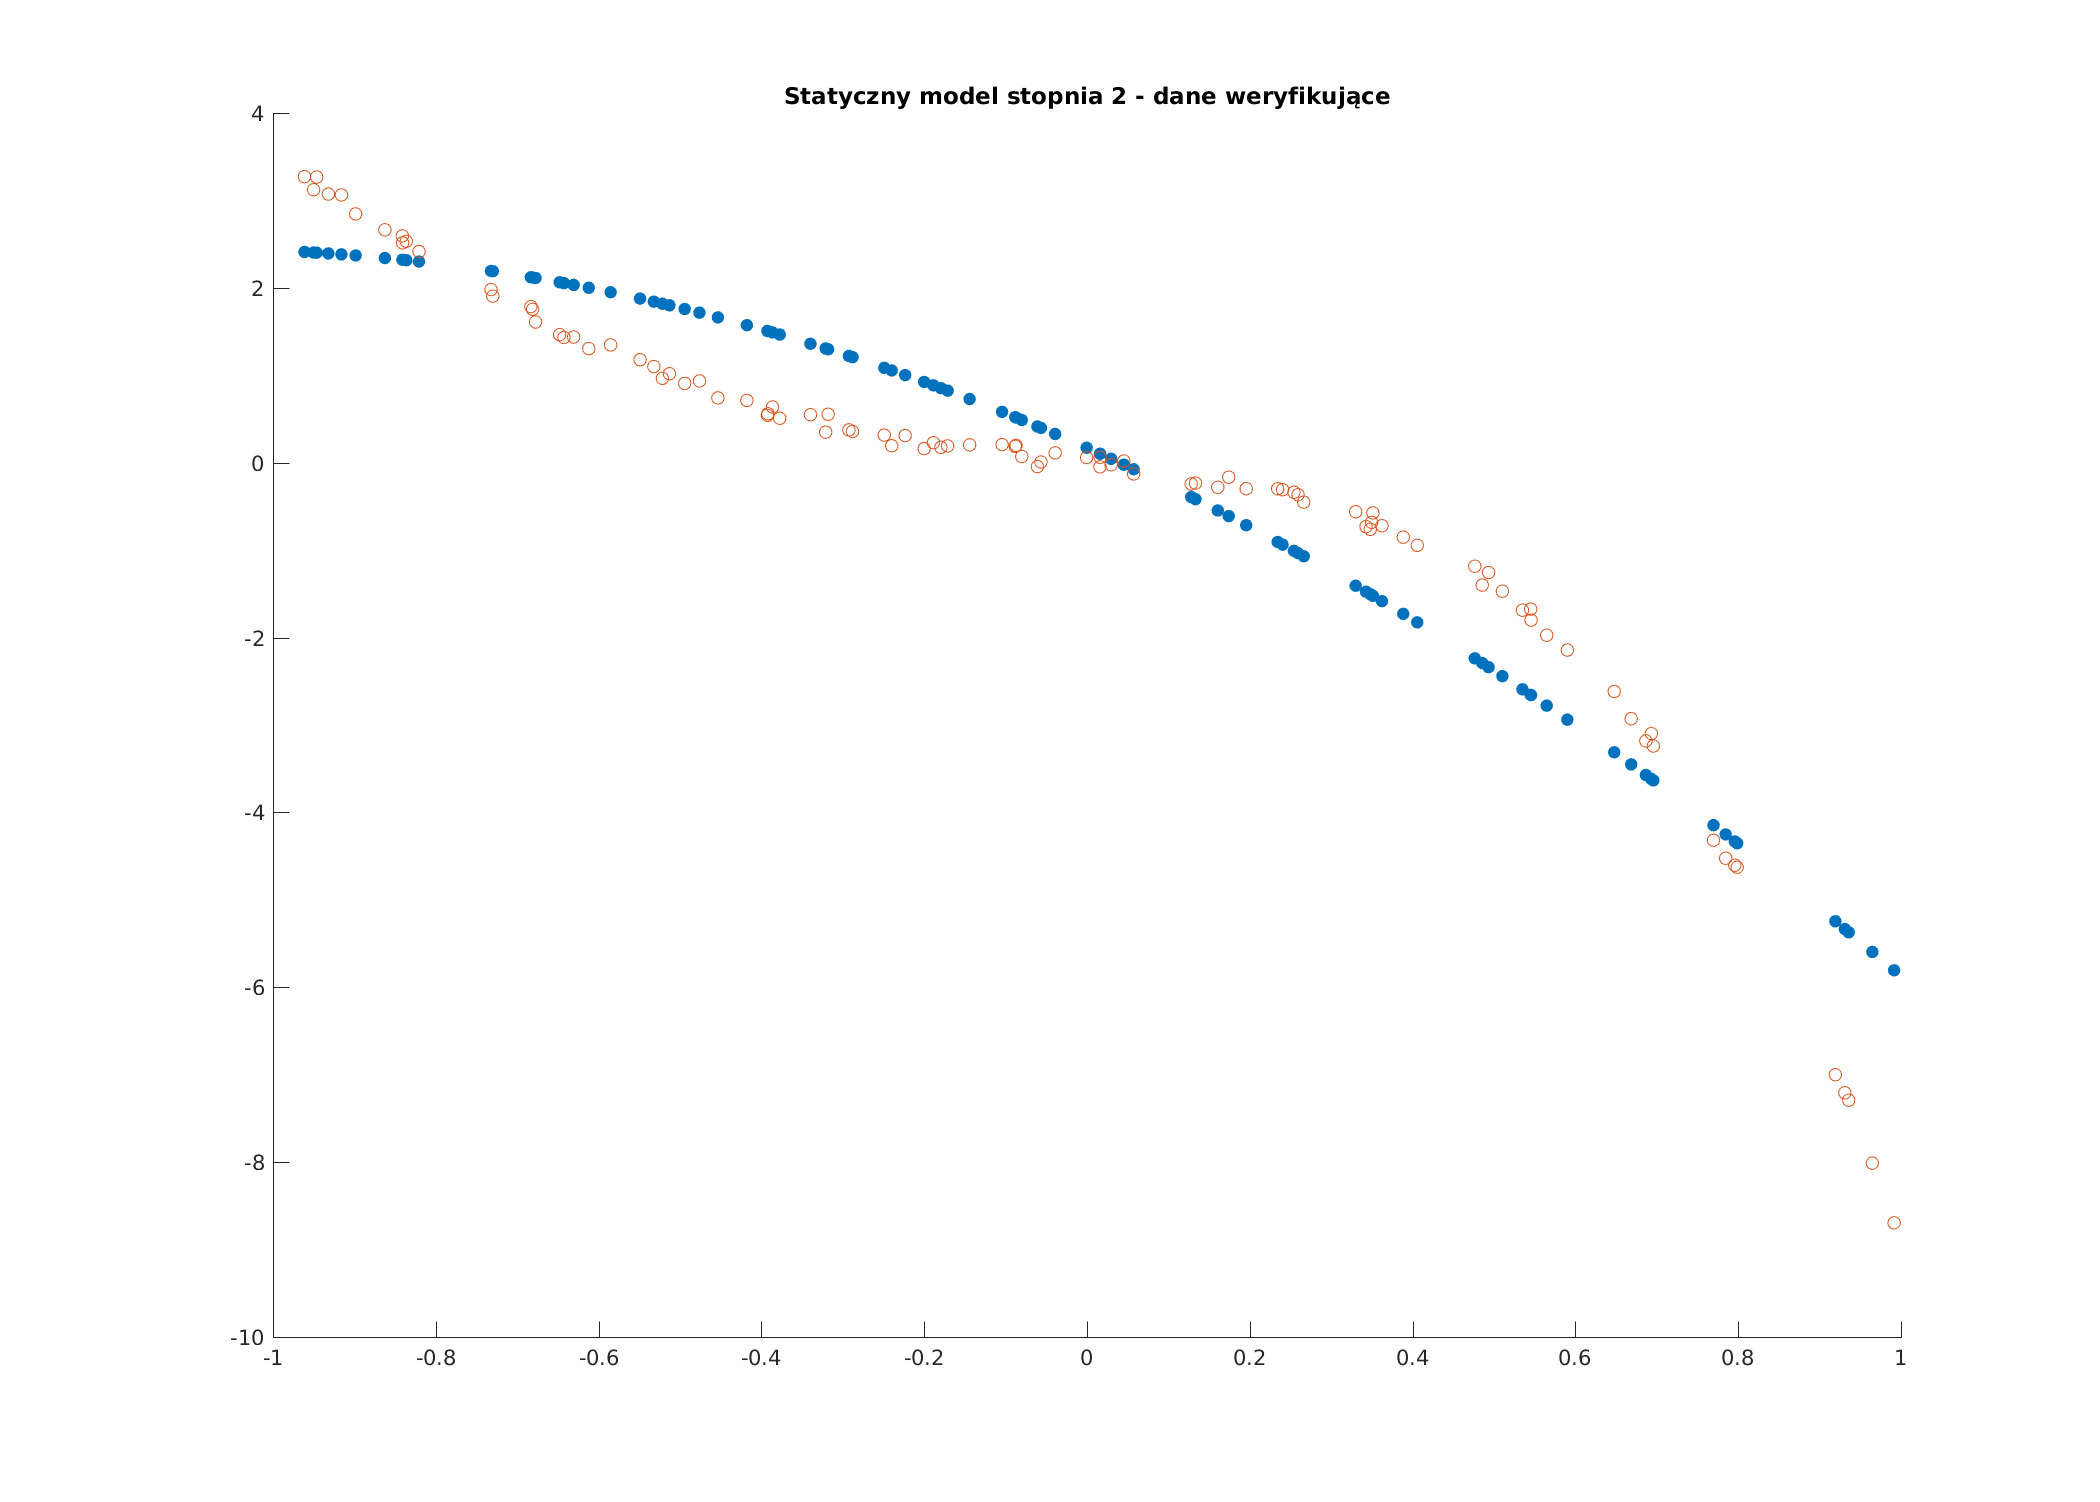
\includegraphics[scale=0.50]{dane_stat_2_wer.png}
\caption{Model stopnia drugiego dane weryfikujące}
\label{}
\end{figure}
\subsubsection{Model stopnia trzeciego}
\begin{figure}[H]
\centering
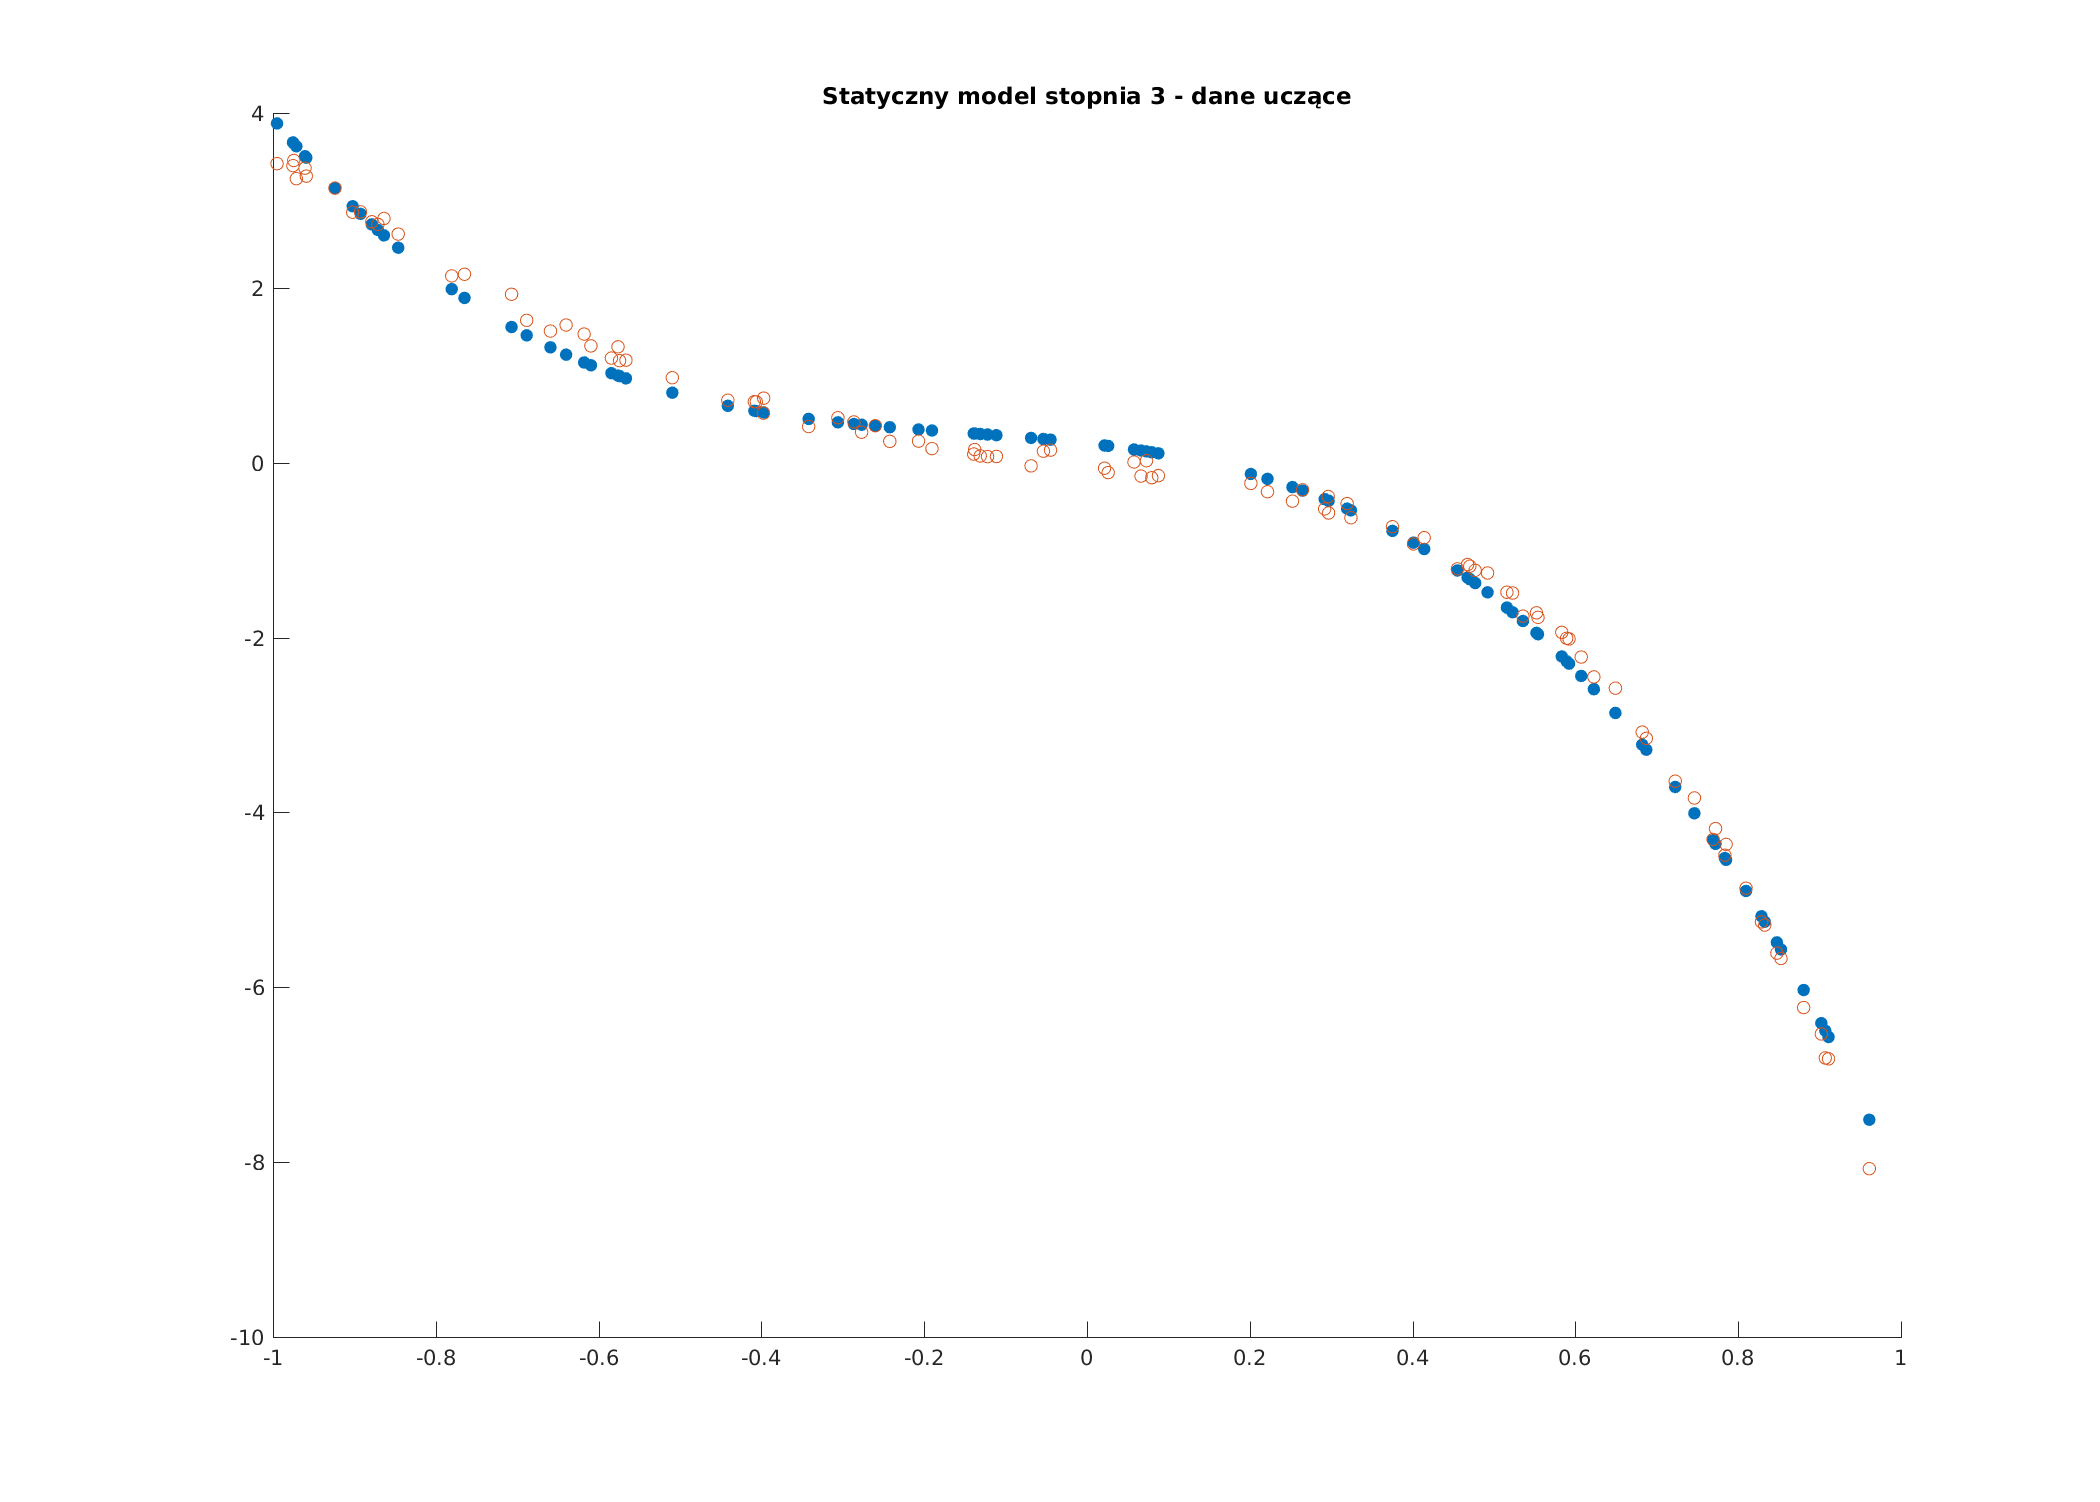
\includegraphics[scale=0.50]{dane_stat_3_ucz.png}
\caption{Model stopnia trzeciego dane uczące}
\label{}
\end{figure}
\begin{figure}[H]
\centering
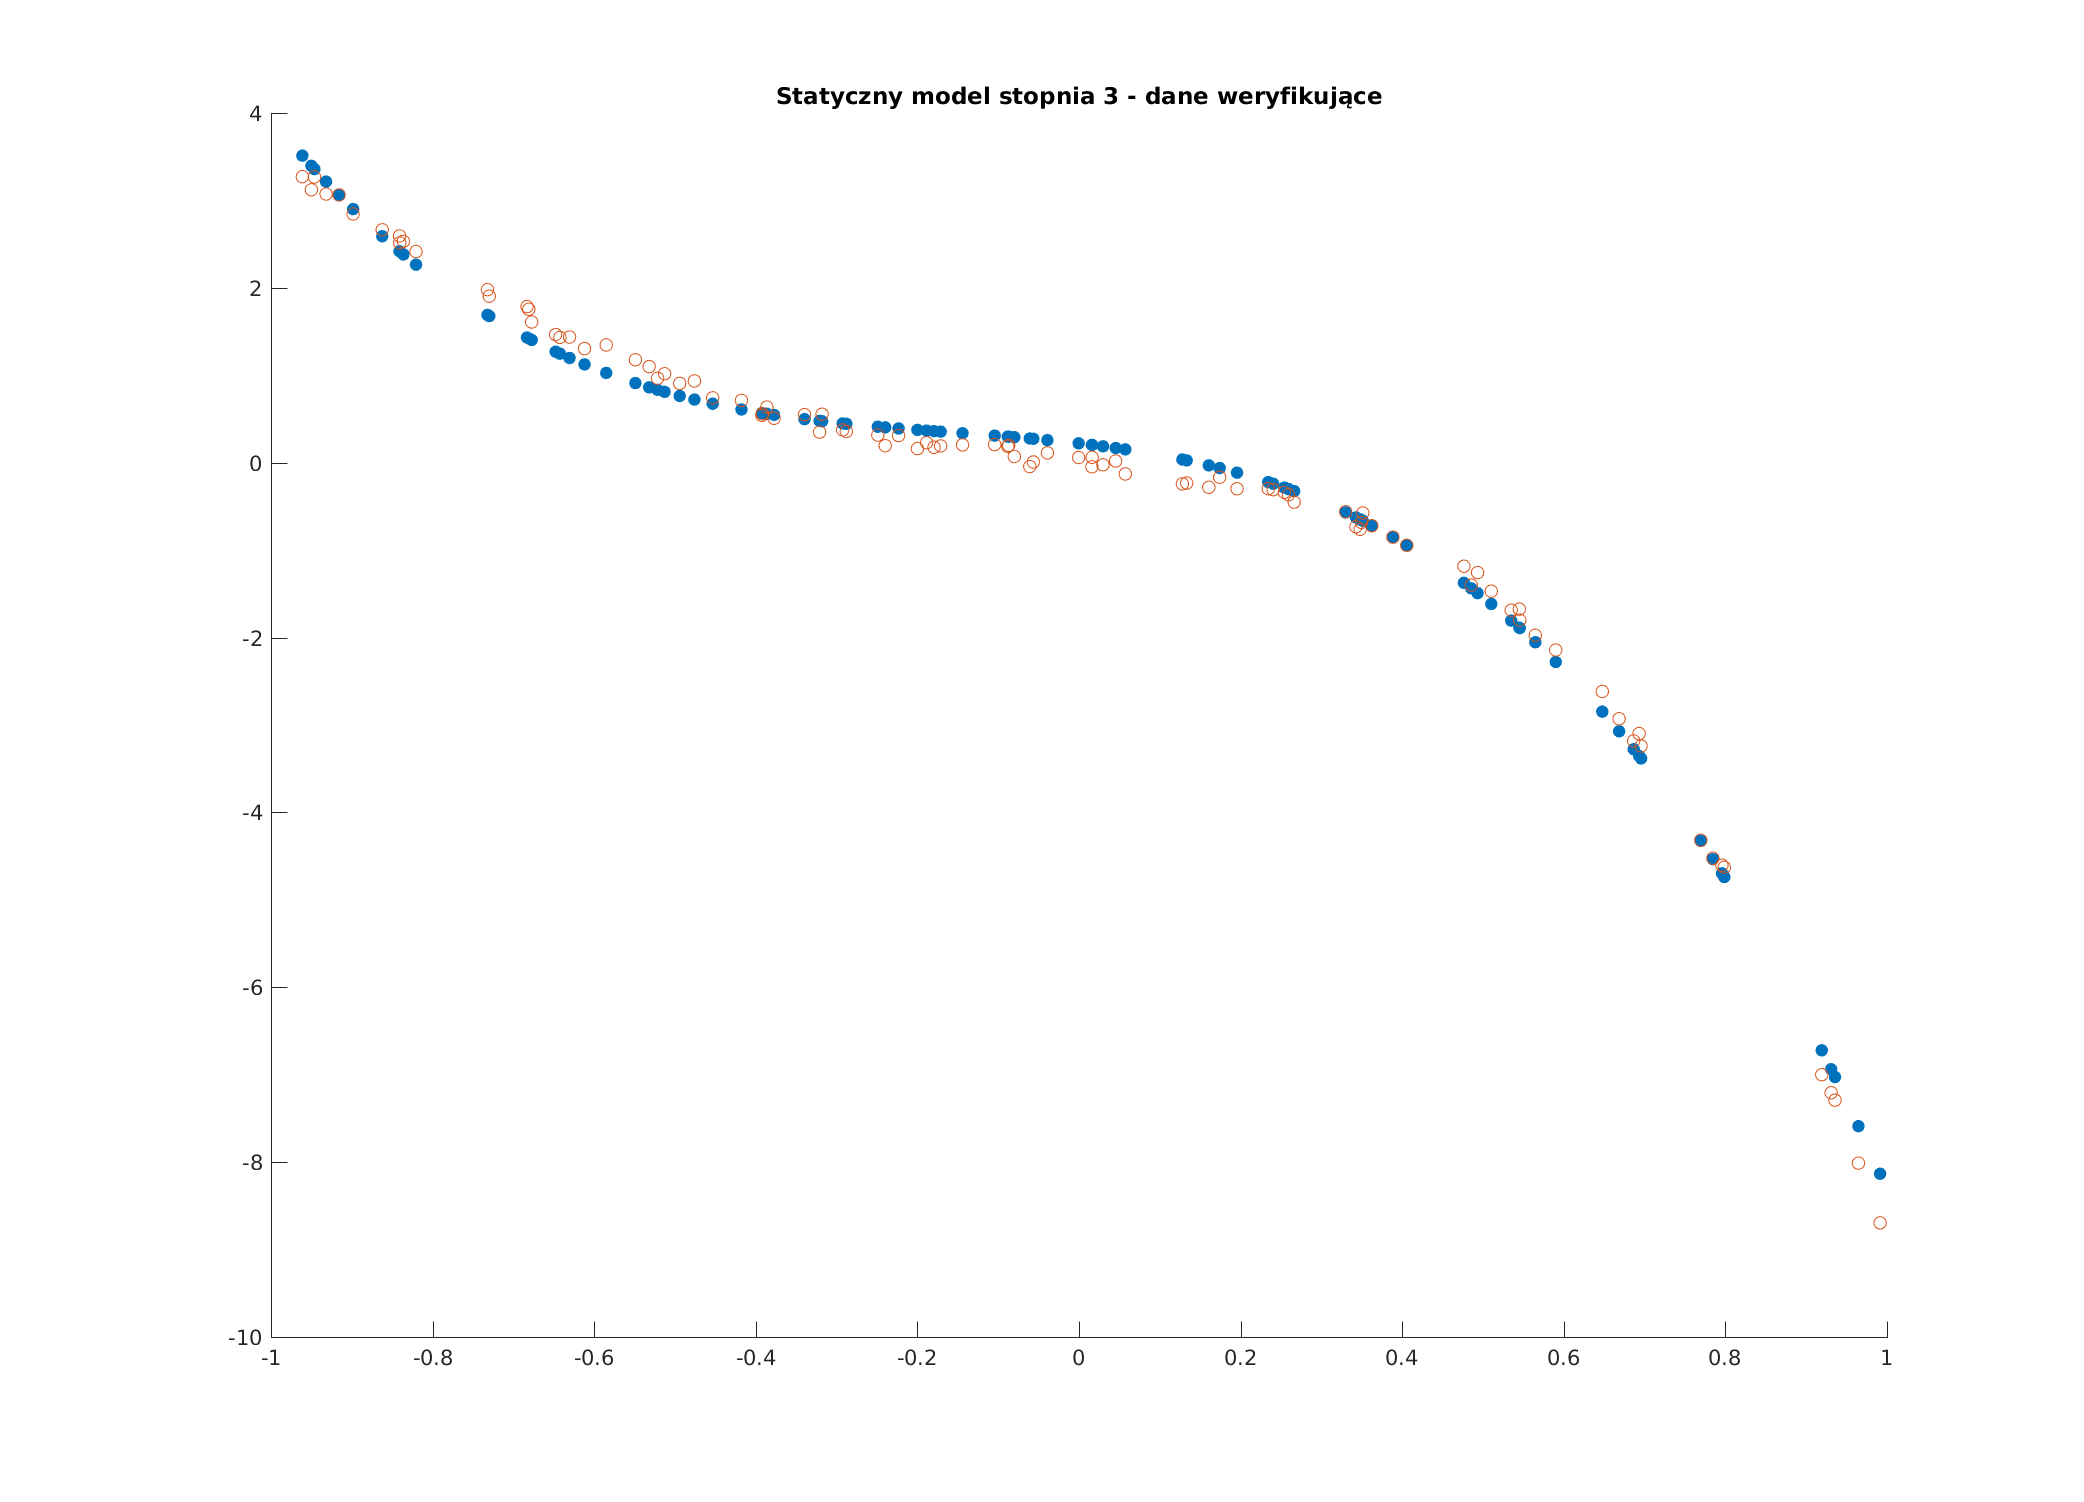
\includegraphics[scale=0.50]{dane_stat_3_wer.png}
\caption{Model stopnia trzeciego dane weryfikujące}
\label{}
\end{figure}
\subsubsection{Model stopnia czwartego}
\begin{figure}[H]
\centering
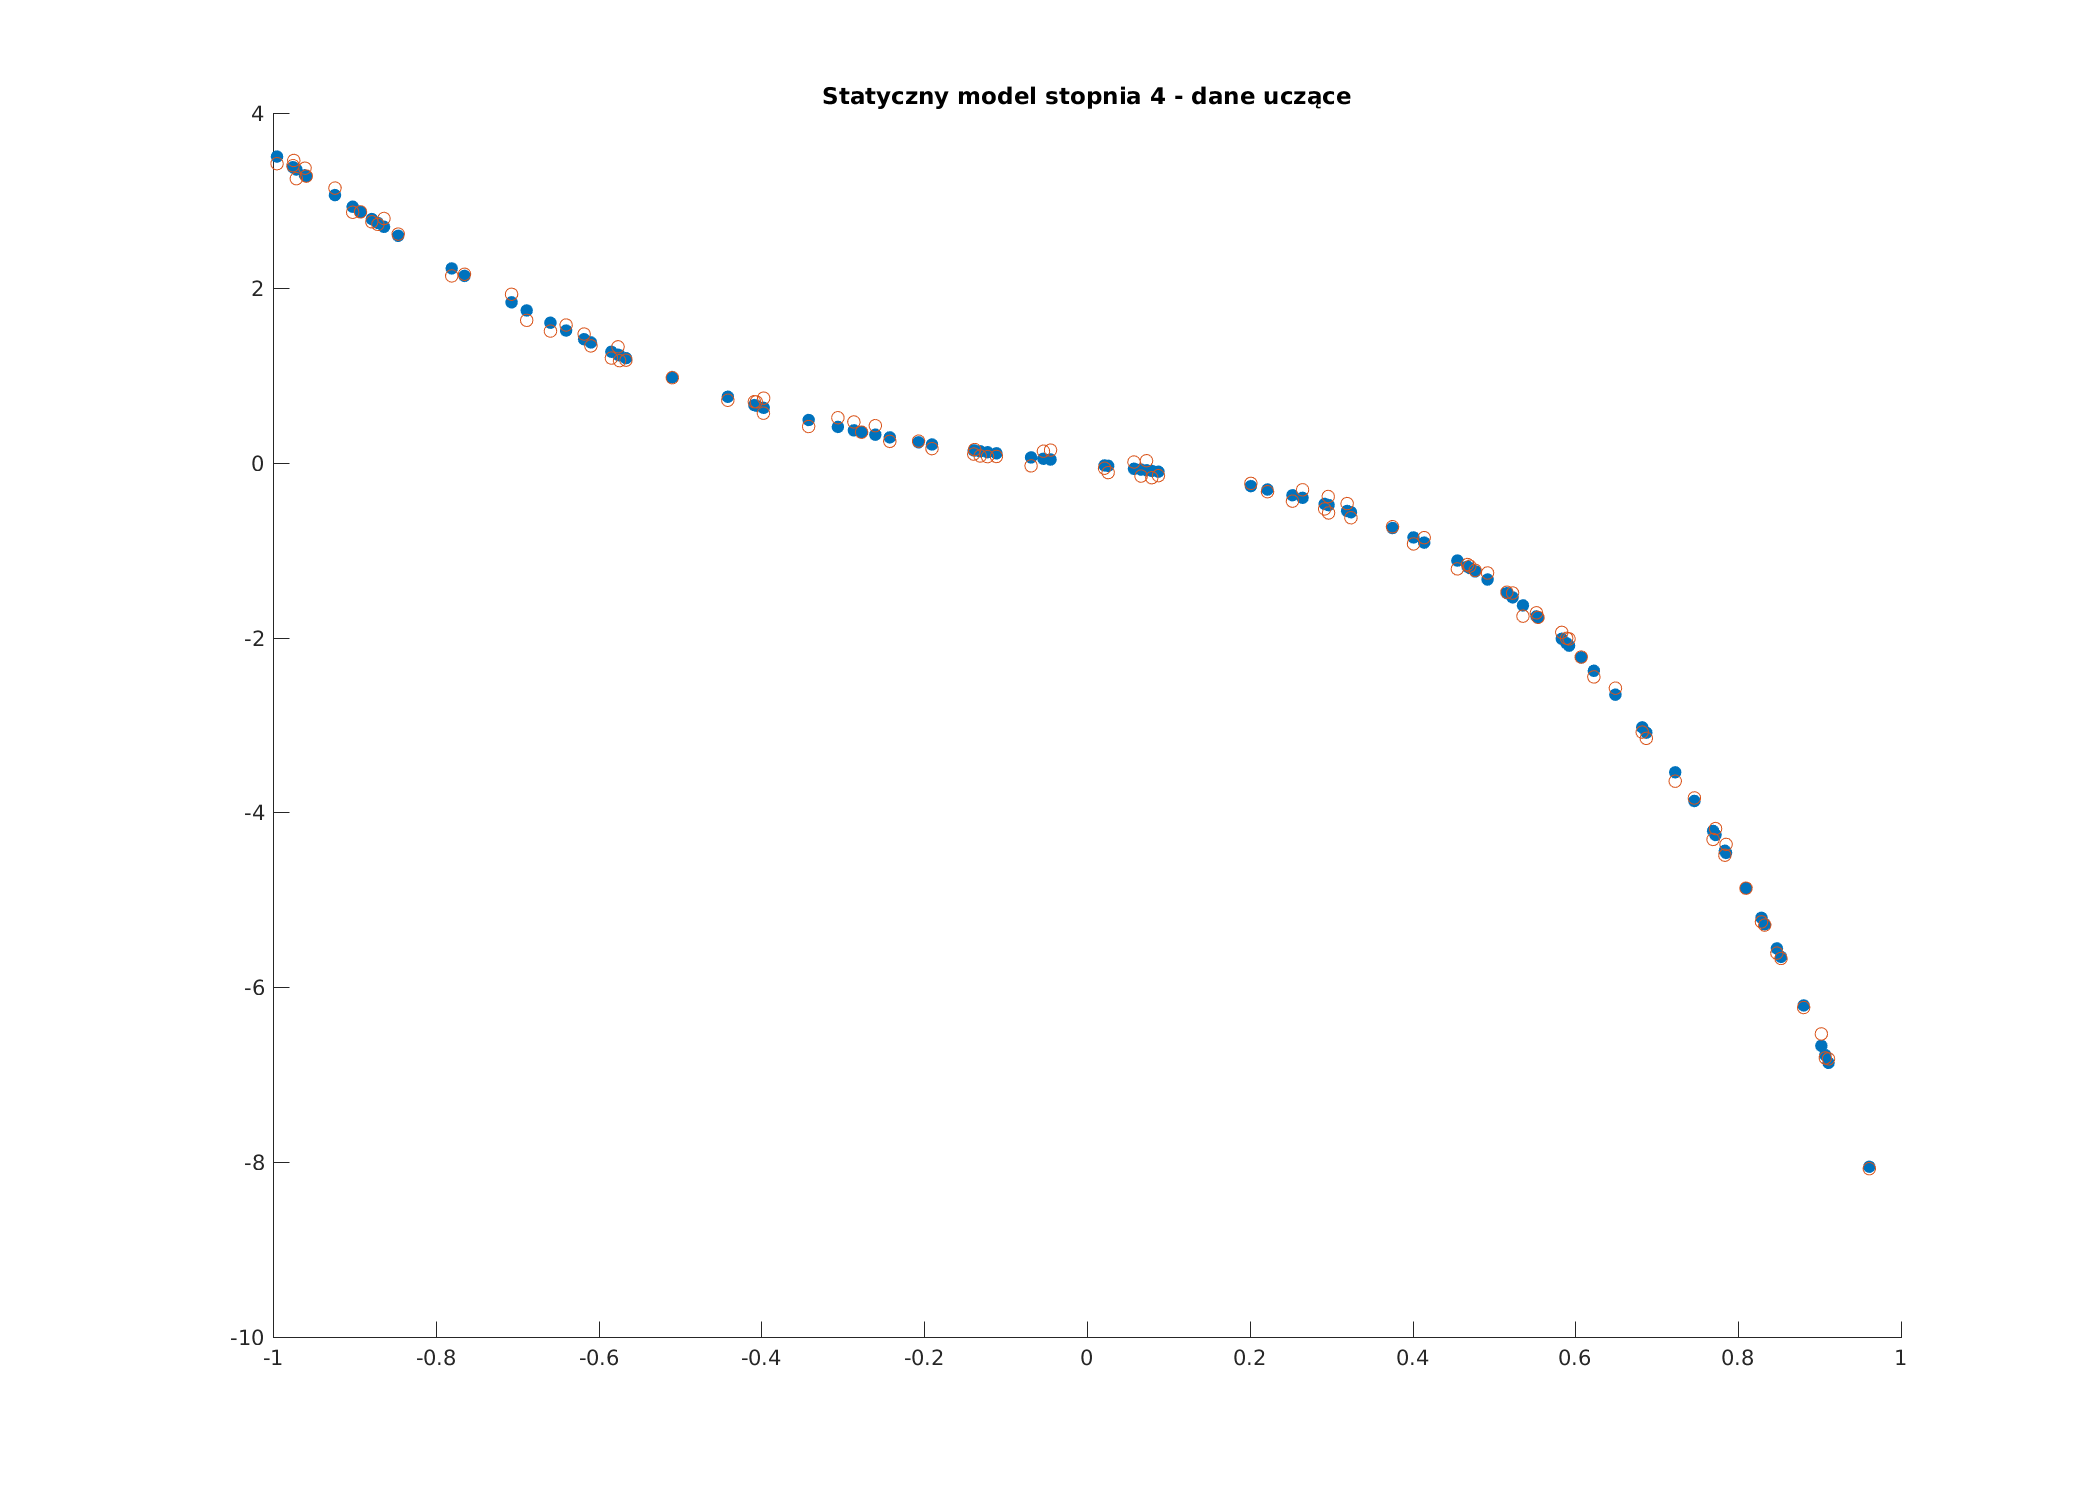
\includegraphics[scale=0.50]{dane_stat_4_ucz.png}
\caption{Model stopnia czwartego dane uczące}
\label{}
\end{figure}
\begin{figure}[H]
\centering
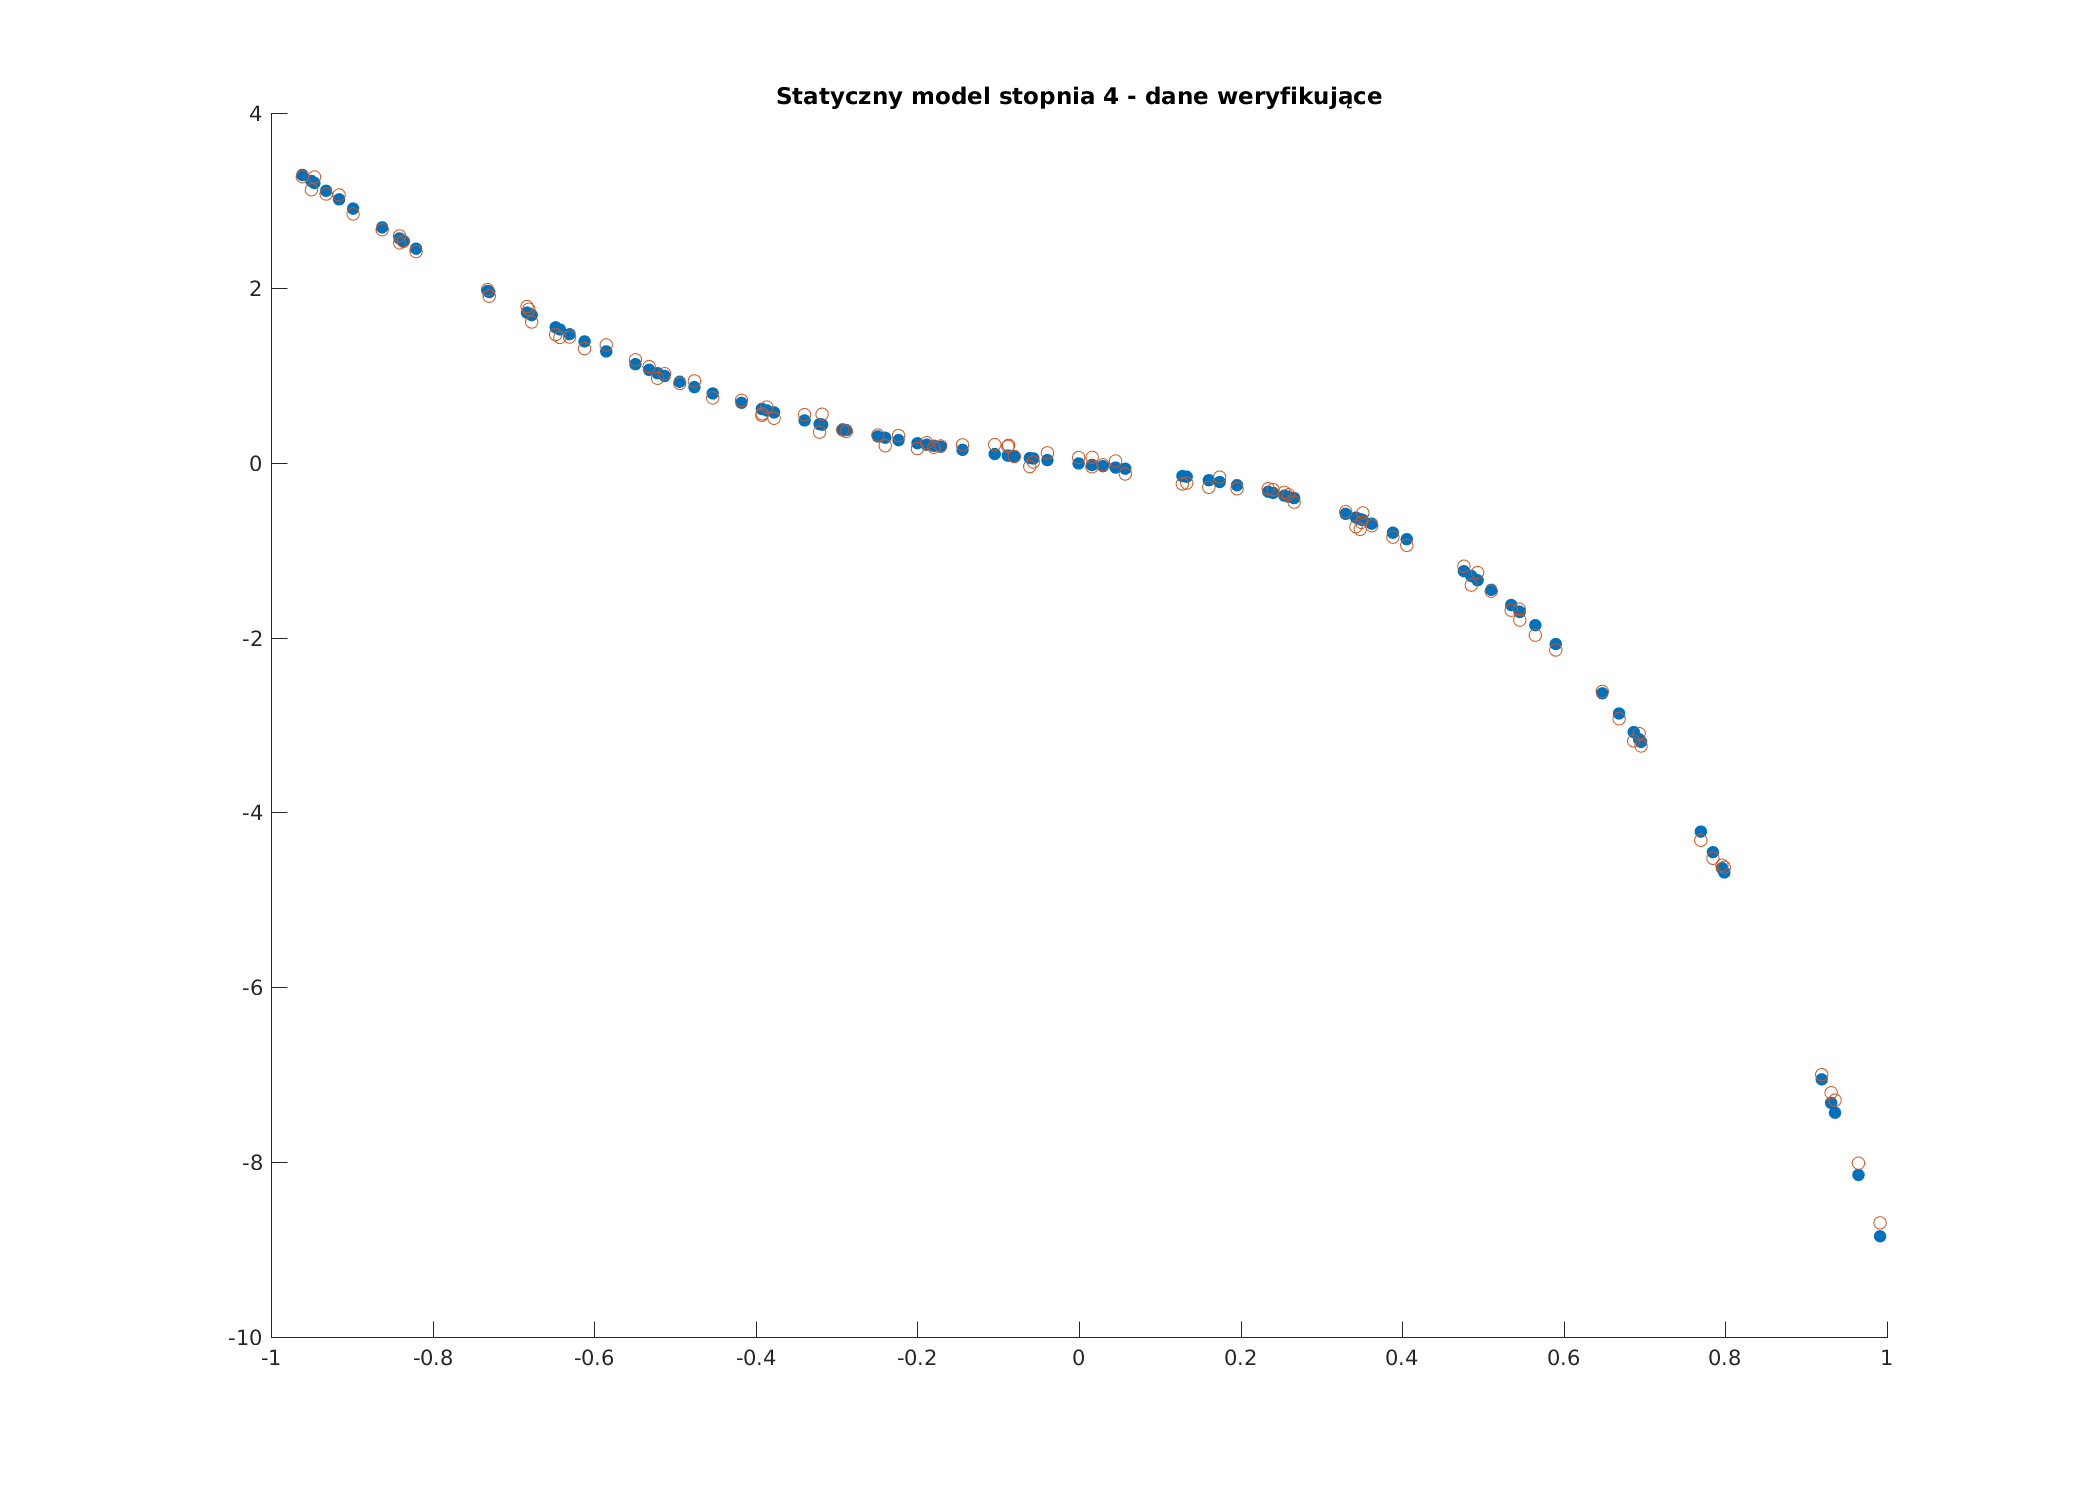
\includegraphics[scale=0.50]{dane_stat_4_wer.png}
\caption{Model stopnia czwartego dane weryfikujące}
\label{}
\end{figure}
\subsubsection{Model stopnia piątego}
\begin{figure}[H]
\centering
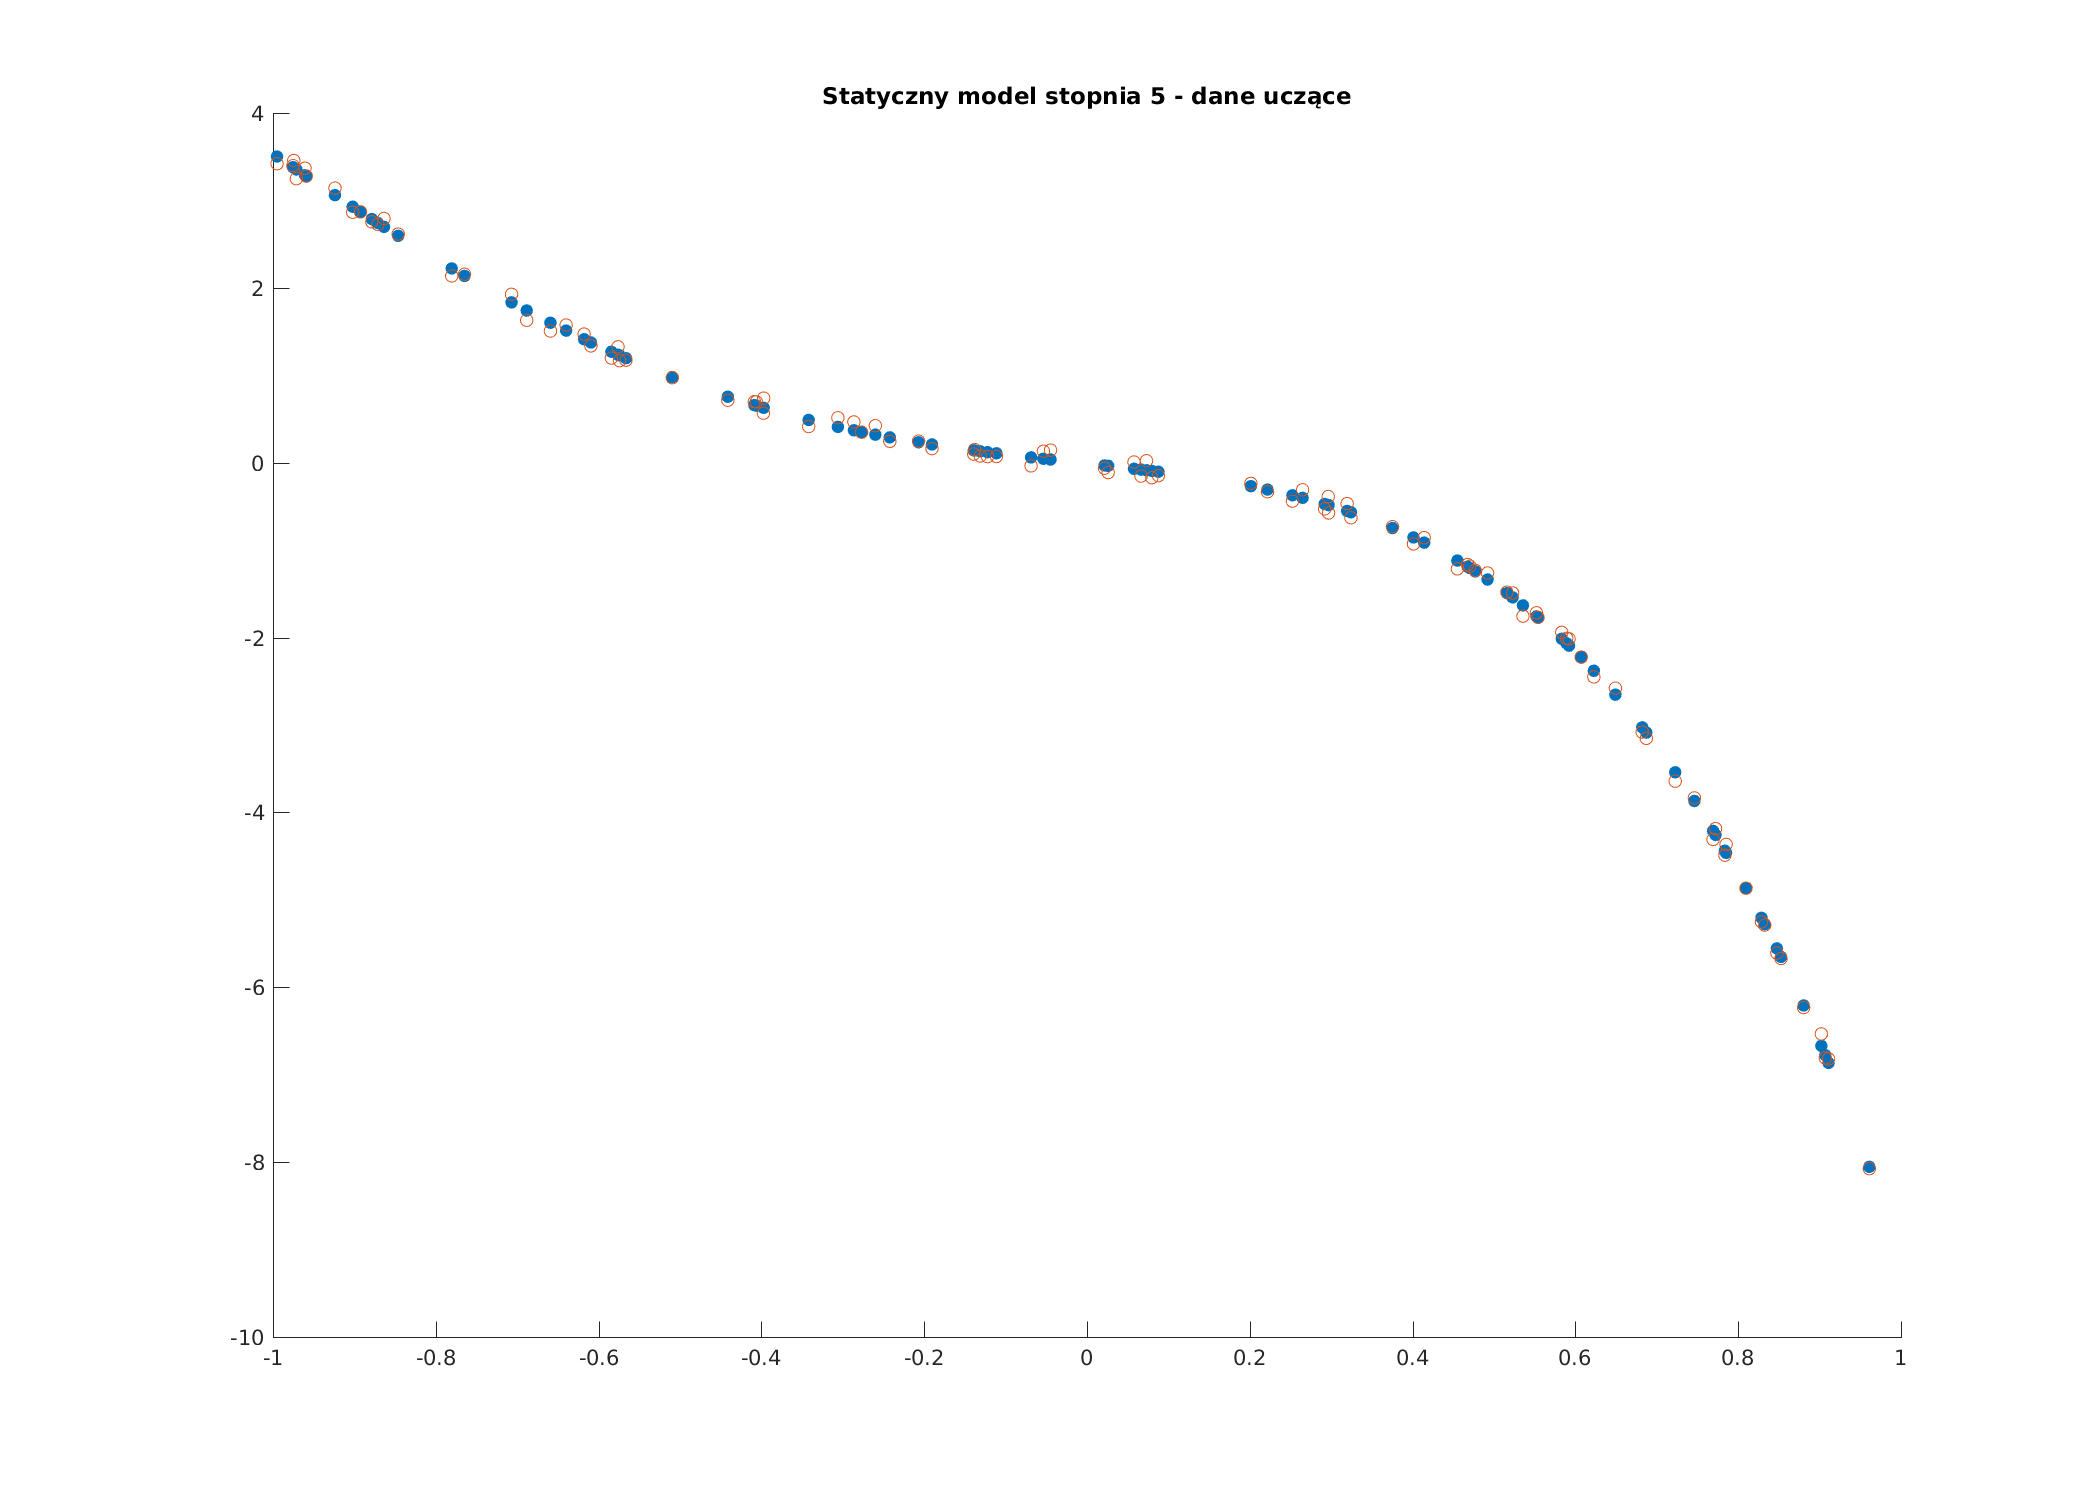
\includegraphics[scale=0.50]{dane_stat_5_ucz.png}
\caption{Model stopnia piątego dane uczące}
\label{}
\end{figure}
\begin{figure}[H]
\centering
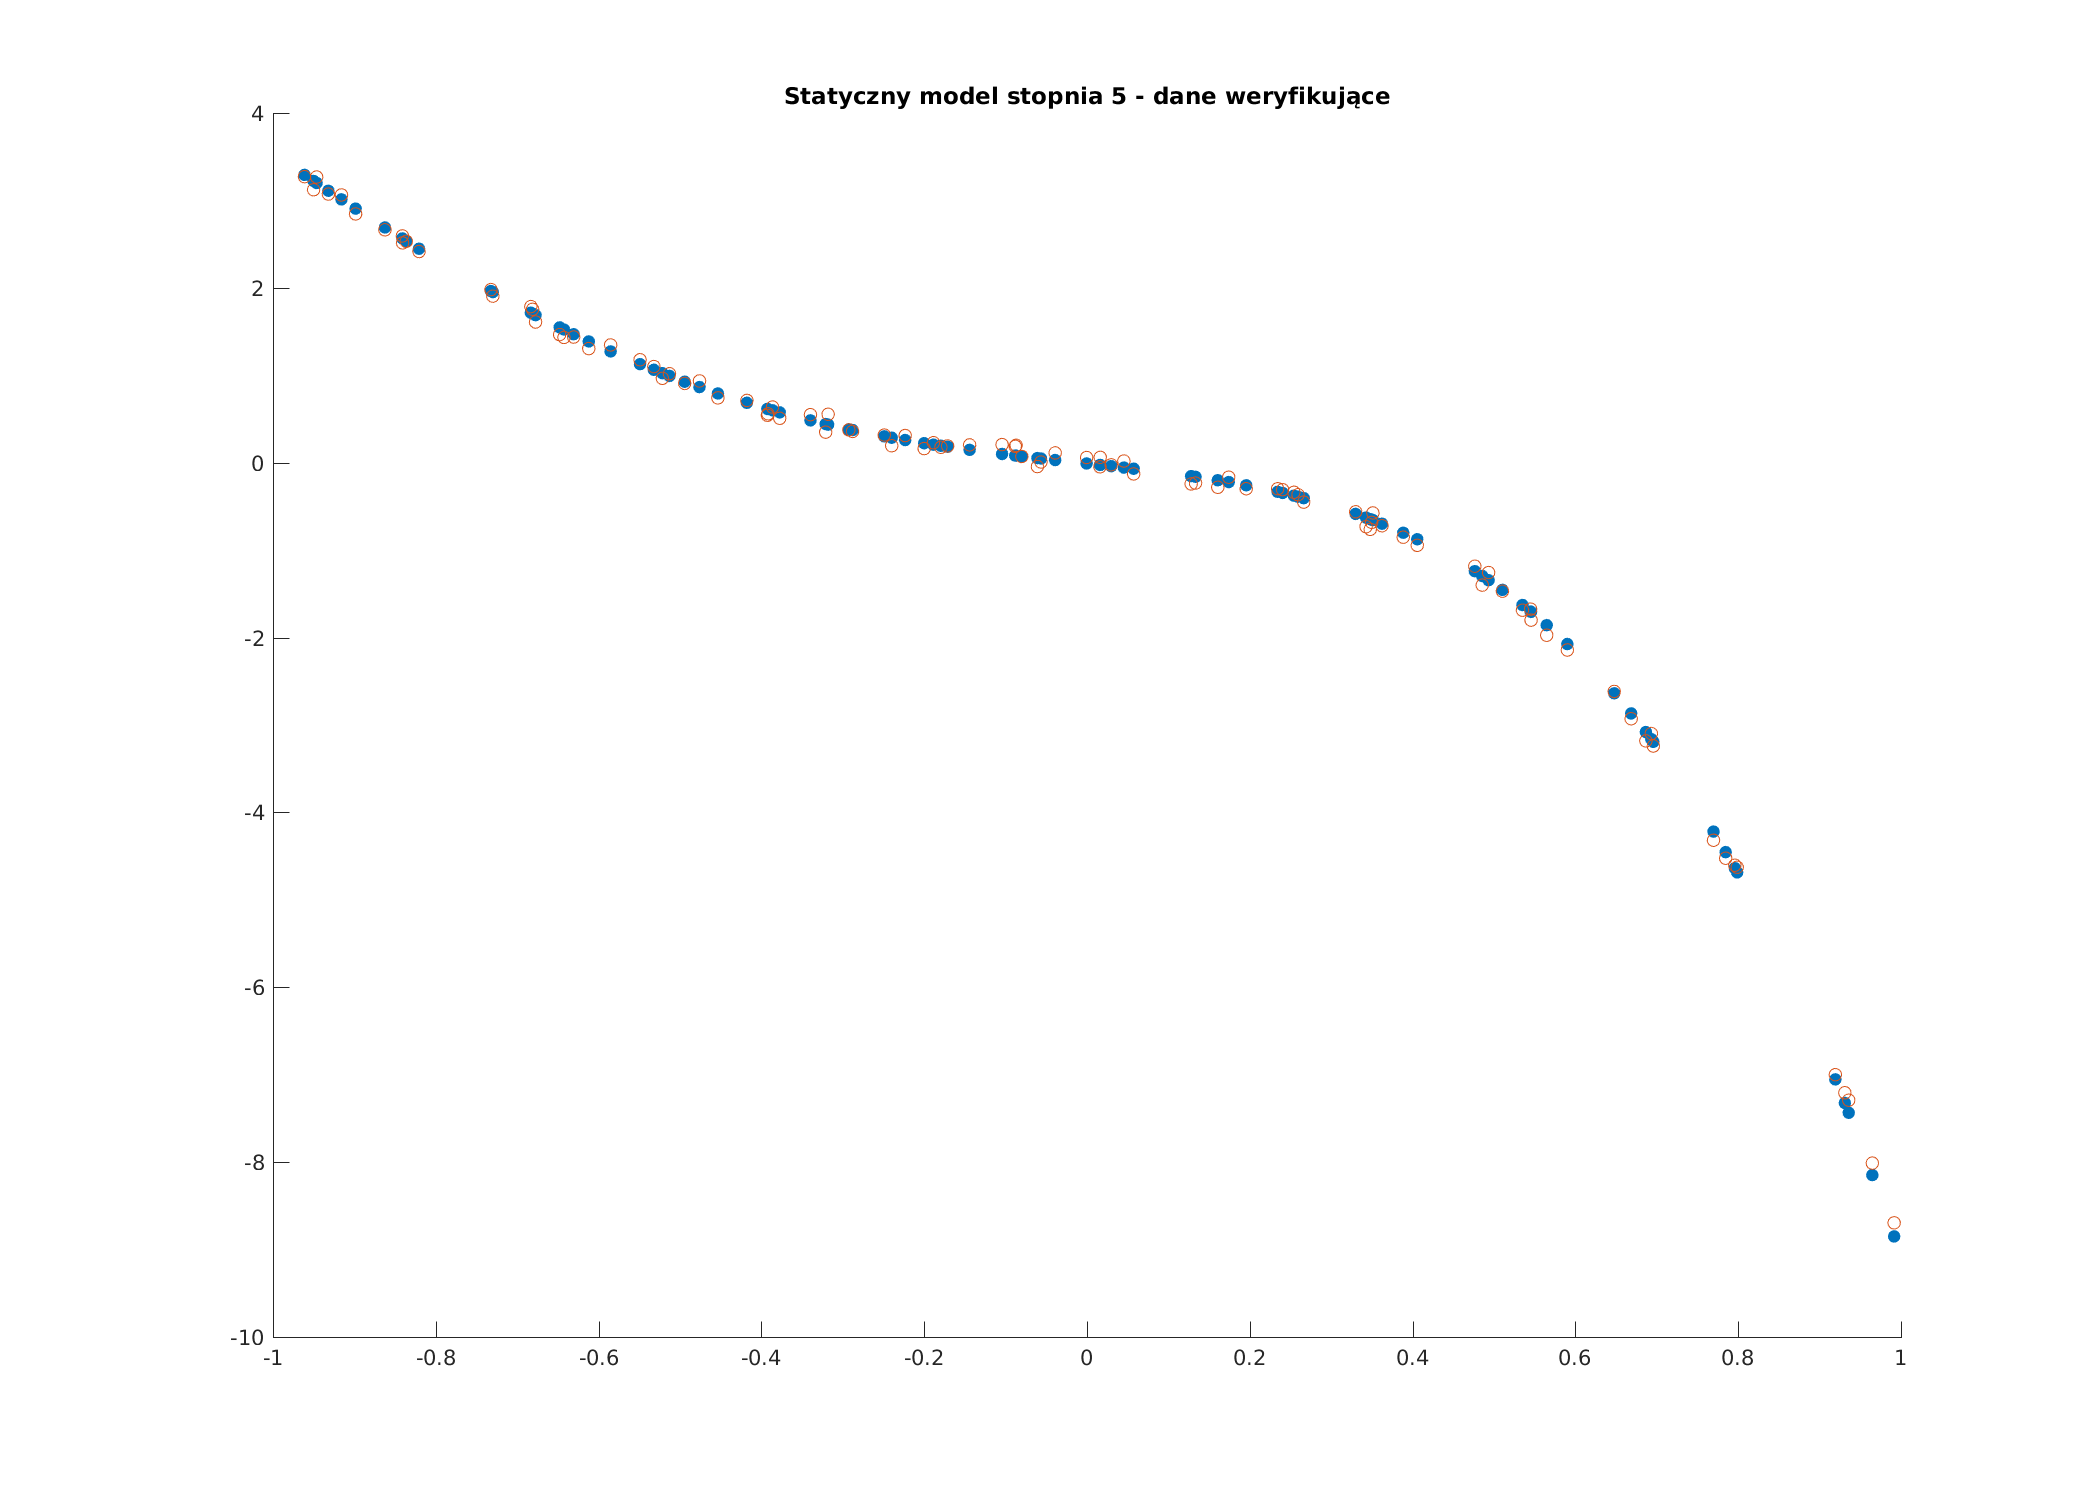
\includegraphics[scale=0.50]{dane_stat_5_wer.png}
\caption{Model stopnia piątego dane weryfikujące}
\label{}
\end{figure}
\subsubsection{Porównanie modeli nieliniowych}
Jako kryterium porównawcze stosujemy błąd dla danych weryfikujących. Zestawienie błedów modeli dla poszczególnych stopni wielomianu przedstawia tabelka: 
\begin{figure}[H]
\centering
\begin{tabular}{|c|c|c|}
\hline
	N & 12 & 13\\
\hline
	1 & 9.432614 & 1.028\\
\hline
	2 & 32 & 33\\
\hline
	3 & 42 & 43\\
\hline
	4 & 52 & 53\\
\hline
	5 & 62 & 63\\
\hline
\end{tabular}
\caption{Zestawienie błedów modeli}
\end{figure}
%dane_ucz_1 9.432614e+01 
%dane_wer_1 1.028000e+02 
%dane_ucz_2 6.186064e+01 
%ane_wer_2 6.537031e+01 
%dane_ucz_3 3.878911e+00 
%ane_wer_3 3.414302e+00 
%dane_ucz_4 4.441852e-01 
%dane_wer_4 4.692886e-01 
%dane_ucz_5 4.441751e-01 
%dane_wer_5 4.703329e-01 
\subsection{Wybór najlepszego modelu}
Najmniejszy błąd dla zbioru weryfikującego występuje w przypadku modelu będącego wielomianem czwartego stopnia, dla stopnia wyższego nastepije pogorszenie modelu. 


\section{Identyfikacja modelu dynamicznego}
\subsection{Reprezentacja graficzna danych dynamicznych}
\subsubsection{Zbiór uczący}
\subsubsection{Zbiór weryfikujacy}
\subsection{Dynamiczne modele liniowe}
\subsubsection{Rzędu pierwszego}
\subsubsection{Rzędu drugiego}
\subsubsection{Rzedu trzeciego}
\subsubsection{Porównianie modeli dynamicznych}
\subsection{Wybór najlepszego modelu}
\subsection{Modele dynamiczene wyznaczne metodą najmniejszych kwadratów} 
\subsubsection{Modele o dynamice pierwszego rzędu}
\subsubsection{Modele o dynamice drugirgo rzędu}
\subsubsection{Modele o dynamice trzeciego rzędu}
\subsubsection{Modele mieszane}
\subsubsection{Porównanie modeli} %tabelka
\subsection{Wybór najlepszego modelu nieliniowego}


\section{Wyznaczanie statycznego modelu nieliniowego}
\subsection{Statyczny model nieliniowy}
\subsection{Reprezentacja graficzna statycznego modelu nieliniowego}



\end{document}